\documentclass[11pt,a4paper]{globis-book}

\usepackage{graphicx}
\usepackage[helvetica]{quotchap}
\usepackage{times}
\usepackage{ethfont}
\usepackage[british]{babel}
\usepackage{longtable}
\usepackage{tabu}
\usepackage{booktabs}
\usepackage[table]{xcolor}
\usepackage{wrapfig}
\usepackage{subcaption}
\usepackage{listings}
\usepackage{fancyhdr}
\usepackage{shadethm}
\usepackage{makeidx}
\usepackage{lipsum}
\usepackage[a4paper,portrait,twoside,inner=3.25cm,outer=3.5cm,top=3.5cm,bottom=4.0cm]{geometry}
\usepackage{hyperref}
\usepackage{globis}
\usepackage{etoolbox}

\renewcommand{\sectfont}{\sffamily\bfseries\Huge}

\setlength{\shadedtextwidth}{\textwidth}
\setlength{\shadeleftshift}{3mm}
\setlength{\shaderightshift}{3mm}
\addtolength{\shadedtextwidth}{-\shadeleftshift}
\addtolength{\shadedtextwidth}{-\shaderightshift}
\setlength{\parindent}{0pt}
\setlength{\parskip}{5pt}

\setcounter{secnumdepth}{5}

%table cells
\definecolor{g}{rgb}{0.5, 0.8, 0.3}
\definecolor{r}{rgb}{0.9,0.3,0.2}
\definecolor{o}{rgb}{1,0.7,0}
\definecolor{i}{gray}{0.7}

\newcommand{\tc}[2]{#2 \cellcolor{#1}}

%fill text next to wrapfig
\newcommand\wrapfill{
	\par 
	\vskip-\baselineskip 
	\WFclear
}

%listings

%no page breaks
\lstnewenvironment{codeex}[1][]%
{
   \noindent
   \minipage{\linewidth} 
   \vspace{0.5\baselineskip}
   \lstset{     
                language = SQL,
                basicstyle=\small\ttfamily,
                frame = trbl,
                tabsize = 2,
                captionpos = b,
                aboveskip = 1em,
                belowskip = 1em,
                xleftmargin = 1em,
                xrightmargin = 1em,
                framexleftmargin = 0.1em,
                framexrightmargin = 0.1em,
                framextopmargin = 0.1em,
                framexbottommargin = 0.1em,
                #1}}
        {\endminipage}
        

%for query set in appendix, allows page breaks
\lstnewenvironment{setq}[1][]%
{
   \lstset{     
                language = SQL,
                basicstyle=\small\ttfamily,
                frame = trbl,
                tabsize = 2,
                captionpos = b,
                aboveskip = 0.6em,
                belowskip = 0.6em,
                xleftmargin = 1em,
                xrightmargin = 1em,
                framexleftmargin = 0.1em,
                framexrightmargin = 0.1em,
                framextopmargin = 0.1em,
                framexbottommargin = 0.1em,
                #1}}{}

\sloppy

\pagestyle{fancy}
\fancyhf{}
\fancyhead[LE,RO]{\sffamily\bfseries\small\thepage}
\fancyhead[LO]{\sffamily\bfseries\small\leftmark}
\fancyhead[RE]{\sffamily\bfseries\small\rightmark}
\renewcommand{\headrulewidth}{0.1pt}
\renewcommand{\footrulewidth}{0pt}

\fancypagestyle{plain}{
   \fancyhf{}
   \fancyfoot[C]{\sffamily\bfseries\small\thepage}
   \renewcommand{\headrulewidth}{0pt}
   \renewcommand{\footrulewidth}{0pt}
}

\hypersetup{
    pdftitle = QENoBI,
    pdfauthor = Patrice Marti,
    pdfsubject = Bachelor Thesis,
		hidelinks,
    plainpages = false,
    bookmarksnumbered = true
}

\raggedbottom

\title{QENoBI - A Node-based Visual Query Builder}
\category{Bachelor Thesis}
\author{Patrice Marti}
\email{$<$martipa@student.ethz.ch$>$}
\professor{Prof. Dr. Moira C. Norrie}
\assistant{Christoph Zimmerli}
\group{Global Information Systems Group}
\institute{Institute of Information Systems}
\department{Department of Computer Science}
\school{ETH Zurich}
\version{}
\date{\today}
\copyrightyear{2015}

\makeindex

\begin{document}

\frontmatter
\maketitlepage
\cleardoublepage
\pdfbookmark{Contents}{toc}

\chapter*{Abstract}
This thesis addresses the question how dataflow programming can be leveraged to create an SQL query builder. The result is QENoBI, a node-based visual SQL query builder that is both exceptionally powerful and easy to use. The thesis discusses different query builder design approaches, highlighting their characteristics and impacts on performance and usability. It then covers the theoretical specification of QENoBI by providing a detailed explanation of all the components. This includes a number of special features, such as subnodes and complete subquery support, that distinguish QENoBI from other query builders. To evaluate the results, a proof-of-concept implementation based on a limited specification is used to verify the concept. The results of the evaluation confirm that the dataflow programming paradigm has considerable advantages over existing query builders.

\tableofcontents

\mainmatter

% Here comes the content


%---------------
%Introduction
%---------------

\chapter{Introduction}
%\newpage
\section{Motivation}

While working at IBM in the early 1970s, Edgar F. Codd invented the concept of the Relational Algebra used to model data stored in relational databases. In the 1971 paper ``A Data Base Sublanguage Founded on the Relational Calculus''\cite{codd1971dbs}, he introduced Alpha as the first database language. Based on Codd's work, Donald D. Chamberlin and Raymond F. Boyce, also working at IBM, developed SQL, one of the first commercial languages to operate on the relational model. Originally conceived to retrieve and manipulate data on IBM's System R, SQL quickly became the most widely used relational data query language and a de facto standard. Despite its popularity, SQL has a number of flaws, some of which caused by the fact that SQL was designed to resemble natural language. This design philosophy lead to arguably absurd constructs such as the IS NOT DISTINCT FROM operator, and, while working well for simple queries, leads to increasingly complex constructs for non-trivial queries. Because of this increase in complexity, tools that partially or completely automate the generation of queries have been investigated by both researchers and commercial companies alike. Due to the widespread use of SQL, most tools are focused on a specific field of application, therefore limiting the complexity, but also power of the tool. Moreover, the inconsistent implementation of the SQL standard by most major database vendors (the exception being PostgreSQL) often leads to tools that are tailored to work with a specific implementation only, producing non-standard SQL code that does not work on other implementations.

During my semester break, I worked with Orbis, a clinical information system produced and marketed by Agfa Healthcare. Orbis is built on top of a relational database backend provided by Oracle and includes a visual query builder used to design queries to be executed on this database. While it is a powerful tool, I was never quite satisfied with it as it seemed overcomplicated and unintuitive to use. At the same time, I was starting to get interested in Blender, an open-source 3D modeling software. One feature that particularly caught my attention, was Blender's approach to certain relatively complicated tasks such as texturing and post-processing, using a node or flow-based programming interface. This choice of interface has proven to be vastly superior to the interfaces used in previous iterations and has therefore been applied to more and more parts of the software.\\
The finding that the node-based programming paradigm can be successfully applied to complex tasks combined with the apparent need for a more capable query builder lead to the idea of a node-based visual query builder, which is the subject of this thesis.

\section{Background}
\label{sec:background}
To investigate the idea of a node-based visual query builder, we first need to establish some background information on the major concepts involved. This includes a definition and some historical background as well as a look at some work previously done in the field.

\subsection{Visual Query Builders}
\label{sec:vis_qb}
\subsubsection*{Definition}
Visual Query Builders are a type of visual programming language designed to simplify the construction of queries on a database. Jeffrey Nickerson defines a visual programming language as a language that uses diagrams in the process of programming, where a diagram is a figure drawn in such a manner that the geometrical or topological relations between the parts of the figure illustrate relations between other objects\footnote{http://www.nickerson.to/visprog/CH2/CH2.HTM}. There are many other definitions, but most of them are very general and could be applied to most query builders that have a graphical interface.

\subsubsection*{History}
The flowchart was introduced by Frank Gilbreth in 1921 as a structured method to model document process flow. However, the use of diagrams to visualize relations between objects can be dated back thousands of years. When computers were introduced in the second half of the twentieth century, they lacked a graphical interface and were therefore unsuited to work with graphical environments such as diagrams. This changed with the introduction of the Xerox Alto developed at PARC which greatly influenced Apple Lisa, the first personal computer to offer a graphical user interface, and more prominently the Apple Macintosh in 1984. However, despite the advances in technology and much interest in the field, visual programming did not find widespread adoption. As a result, the vast majority of programs are still written in a traditional text-based programming language.

\subsubsection*{Examples}
To get an idea of the current state of the art of visual query builders, we will take a look at a list of examples. These include commercial products as well as solutions presented in research papers. The examples presented in this section are meant as an overview rather than a thorough analysis of the field but will also be used in Section~\ref{sec:test_set} to derive a set of requirements used to define the outline of the tool presented in this thesis.

\paragraph*{EasyQuery\footnote{http://devtools.korzh.com/easyquery}}
EasyQuery is a commercial product developed by Korzh.com, located in Kyiv. It is presented as an ``ad-hoc visual query builder [that] allows [the user] to construct a query visually: simply by assembling a phrase in natural language.''

\begin{figure}[h]
  \centering
  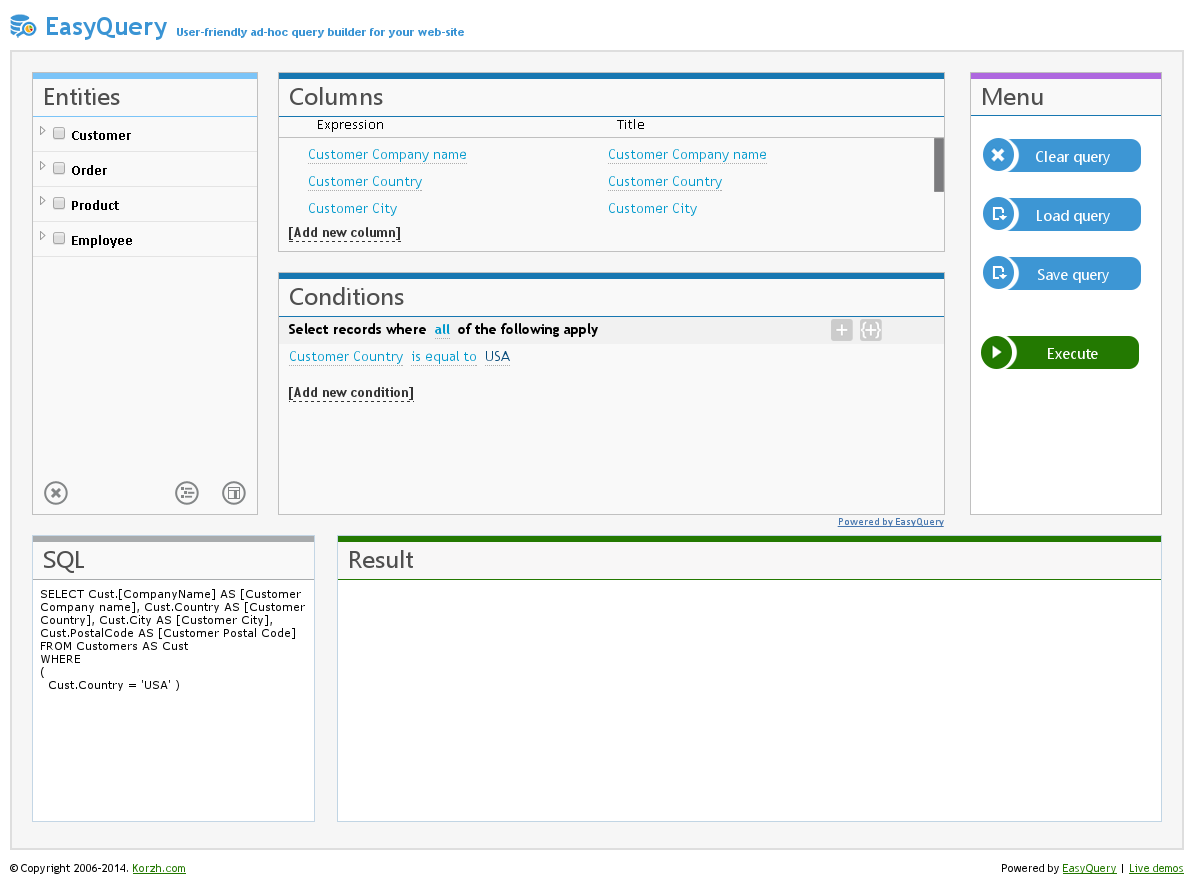
\includegraphics[width=\textwidth]{resources/EasyQuery.png}
  \caption{A screenshot of EasyQuery, showing its form-based interface}
  \label{fig:easyquery}
\end{figure}

The user interface consists of lists for entities, columns and conditions as well as two output text containers for the produced query and optionally the results from its execution. A screenshot of the interface is shown in Figure~\ref{fig:easyquery}. As such, according to our definition, EasyQuery cannot be considered a visual programming language, as it does not include diagrams or figures of any sorts. In spite of this, EasyQuery has a few unique features lacking from the other query builders examined, such as an implicit join notation, partial subquery support and a powerful, tool-assisted schema declaration. The latter includes information not only about the tables but also their relations, therefore enabling the automatic joining of tables when necessary. For instance, if a user adds a condition comparing two columns originating from different tables, EasyQuery will automatically attempt to derive a join order, based on the foreign keys defined in the schema declaration. This feature is targeted at novice users unfamiliar with the concepts of relational databases. This comes at a cost however, greatly reducing the amount of control the user has over the structure of the query and limiting the number of queries that can be described. One such limitation is the inavailability of self-joins, as the query builder is unable to distinguish it from a simple comparison of two columns in the same table.

\paragraph*{ExtJS\footnote{http://www.cfsolution.de/qb}}
Most commercial general-purpose query builders put the focus on joining the tables by means of visually connecting nodes. One examples is ExtJS, developed by cfsolutions.

\begin{figure}[h]
  \centering
  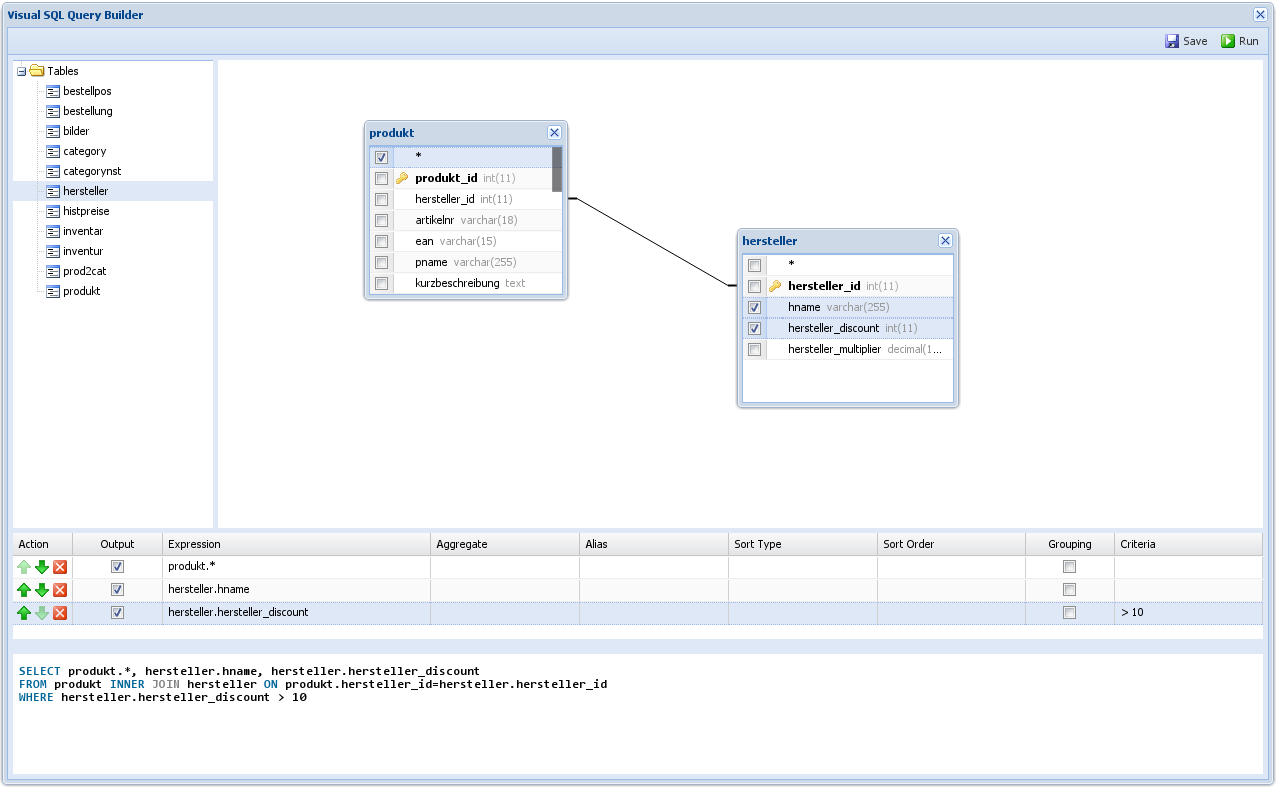
\includegraphics[width=\textwidth]{resources/ExtJS.png}
  \caption{A screenshot of ExtJS, showing its table-based interface}
  \label{fig:extjs}
\end{figure}

Tables are represented as nodes, containing a list of the columns present in the table. A checkbox is used to designate whether a column is in the projection. Tables can be joined by dragging a column onto another one, resulting in a visual indicator, as seen in the screenshot in Figure~\ref{fig:extjs}. Due to the use of nodes and connections between them, ExtJS and similar query builder satisfy our definition of a visual programming language. However, projected columns are displayed in a list with the option to apply expressions, aggregate functions, aliasing, sorting and grouping as well as conditions, all using text fields. This non-visual approach is very powerful, allowing the user to design complex queries. However, it is very difficult to maintain type safety and therefore, it is possible to create syntactically incorrect queries in many different ways.

\paragraph*{DFQL}
Dataflow Query Language is a visual query language proposed in a 1994 paper by Gard J. Clark and C. Thomas Wu\cite{clark1994dfql}. It is based on the concept of flow-based programming allowing incremental construction of queries.

\begin{figure}[h]
  \centering
  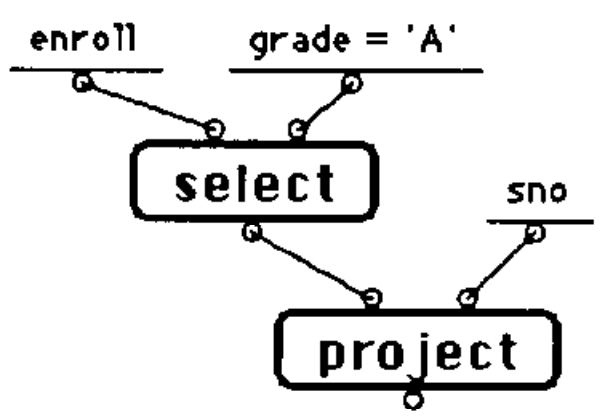
\includegraphics[width=0.4\textwidth]{resources/DFQL.png}
  \caption{A simple query in DFQL}
  \label{fig:dfql}
\end{figure}

DFQL is very close to the idea resulting from the motivation, using dataflow programming to access data on relational databases. However, DFQL is not a query builder in the classic sense, as it is intended as a standalone query language. Unlike SQL, it is a strict implementation of the relational algebra and relationally complete. It maintains relational closure, meaning that the output of every node is again a relation, leading to a very intuitive way of constructing subqueries. Inputs that are not relations, such as conditions and projections are entered in text form, represented as a straight line in the diagram. Figure~\ref{fig:dfql} shows a simple query expressed in DFQL. This approach is conceptually similar to conditions in ExtJS, albeit more tightly integrated into the interface. It shares the weaknesses and strengths of this approach of being very powerful while allowing the creation of syntactically incorrect queries. DFQL makes strong use of the dataflow paradigm, allowing the grouping of multiple nodes into subnodes. This feature is also present in Blender and was therefore a part of the original idea from the very beginning.

\paragraph*{Konduit} Konduit is a query builder for SPARQL. It was introduced in a 2010 paper by Oszk{\'a}r Ambrusoszkar, Knud M\"oller and Siegfried Handschuh\cite{ambrus2010konduit}. SPARQL operates on RDF data used to represent data in the semantic web. However, with the adoption of Nepomuk as part of KDE, the semantic data concept also found its way onto the desktop. Konduit aims to assist users in building queries on this data. The paper examines different user interface approaches that are similar to EasyQuery in that they are based in lists as opposed to diagrams. Therefore, Konduit is not a visual query builder according to our definition. Nonetheless, the graph-like structure of RDF queries result in interesting approaches that can also be applied to SQL querying.

\paragraph*{MDDQL} Meta-Data Driven Query Language is a visual query language described in a 2000 paper by E. Kapetanios, M. C. Norrie, D. Fuhrer-Stakic\cite{kapetanios2000mddql}. MDDQL explores the idea of using semantic data to simplify query generation on large schemas. Semantic data is represented in a way similar to RDF using domains of interest and operations. While MDDQL is not a general-purpose SQL query builder, the concept of using semantics to assist query generation could also be used for SQL.

\subsubsection*{Discussion}
Commercial and academic research has spawned a number of different visual query builder concepts, each with their own strengths and weaknesses. The flaws and inconsistencies of SQL make it very challenging to create a tool that is both powerful and intuitive to use, while ensuring correctness of the query. EasyQuery shows almost perfect correctness at the cost of significantly reduced power and a less visual interface. ExtJS is a more visual as well as powerful approach, but does not feature a particularly intuitive interface either in that it is generally not suited for novice users. DFQL on the other hand is significantly more powerful, featuring complete subquery support while relying on a much simpler user interface, therefore improving usability. It shares the correctness weaknesses of ExtJS and additionally, the fact that it does not produce SQL greatly reduces its practical impact. Nonetheless, the quick analysis of DFQL reveals that the dataflow programming offers some significant benefits. Additionally, using semantic information to assist the query generation process could be very valuable as shown by Konduit and MDDQL.

\subsection{Dataflow Programming}
\subsubsection*{Definition}
\label{sec:dfp}
Dataflow programming is a programming paradigm that emphasizes the flow of data between processes rather than the execution of statements in the imperative paradigm used by most programming languages today. Dataflow-based applications are defined as a network, i.e. a graph of black-boxed processes that exchange data across predefined connections. This network is usually defined in the form of a diagram, making dataflow programming a visual programming paradigm. Moreover, since the program is essentially reduced to sets of processes and dependencies, it is effectively language-independent. Dataflow programming shares some features of functional programming languages in that the nodes are usually stateless, meaning that the output of a node depends entirely on its inputs.

Metaphorically speaking, dataflow programming can be described as an assembly line, where workers modify some form of information packets that are moved between workers using the assembly line. In an actual program, the workers are represented by nodes that exchange data by message passing along predefined channels, which represent the assembly line. In comparison, traditional imperative programming can be imagined as a single worker moving between tasks.

\subsubsection*{History}
Dataflow programming was pioneered by John Larry Kelly Jr., Carol Lochbaum and Victor A. Vyssotsky at Bell Labs. In 1961 paper ``A Block Diagram Compiler''\cite{kelly1961block}, they introduced the BLODI programming language as a way to model programs in a manner similar to block diagrams used by engineers. As dataflow programs focus on the flow of data, they are inherently parallel and as a result, subsequent dataflow languages were often developed at supercomputer labs. One of the most prominent dataflow languages of that time period is SISAL. More recently however, the concept has attracted mainstream attention, resulting in a number of new projects. One of these projects is NoFlo, a dataflow-based development environment started by Henri Bergius in 2013. In light of these developments, a number of major software companies such as IBM, Facebook and Microsoft, have announced new products based on the concept.

\subsubsection*{Examples}
\paragraph*{SISAL}
Streams and Iteration in a Single Assignment Language\cite{mcgraw1983sisal} is a general-purpose single assignment programming language based on the dataflow programming paradigm. Defined in 1983 by James McGraw et al. and released in 1986, it was a very popular language used to implement algorithms to be executed on supercomputers due to its very high performance. SISAL is not a visual language but instead features a Pascal-like syntax. The program code is subsequently translated into a graph representation which can be executed directly or translated into C code.

\paragraph*{NoFlo\footnote{http://www.noflojs.org/}}
NoFlo is an open-source project lead by Henri Bergius aiming at creating a JavaScript programming environment based on the concepts of flow-based programming. Flow-based programming is a form of dataflow programming that focuses on data stream processing.

\begin{figure}[h]
  \centering
  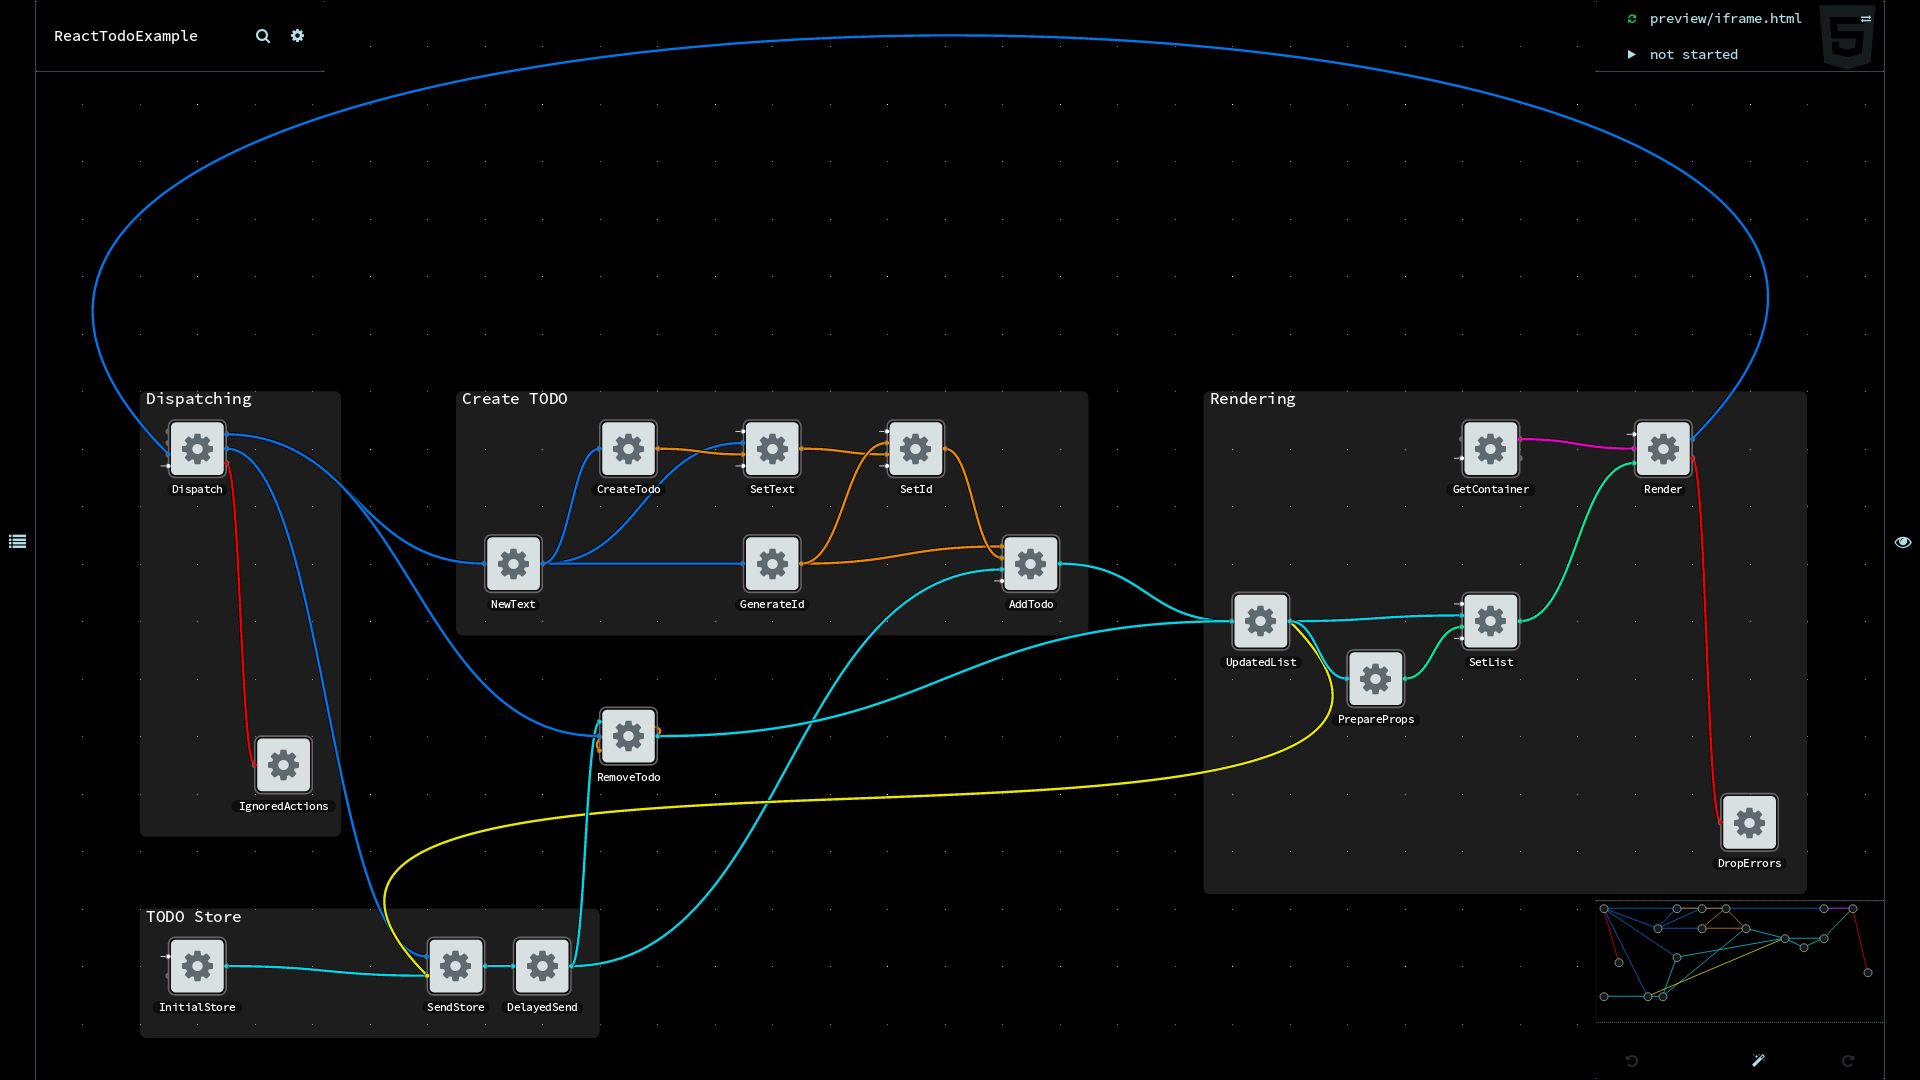
\includegraphics[width=\textwidth]{resources/NoFlo.png}
  \caption{A NoFlo application}
  \label{fig:noflo}
\end{figure}

The first commit was pushed in June 2011 and in 2013, a Kickstarter campaign was started to secure funding for the development of a graphical interface to NoFlo, titled NoFlo-UI. The campaign was successful not only in securing the funds but also spreading the word about the project and flow-based and dataflow programming in general. NoFlo differs from flow-based programming in a number of aspects as described by John Paul Morrison\footnote{http://www.jpaulmorrison.com/fbp/noflo.html}, the inventor of flow-based programming. It suffices to say that NoFlo focuses on application design rather than data streams.

\paragraph*{Blender}
Blender is a professional open-source 3D computer graphics software. It supports a variety of features such as 3D modeling, animating, texturing and composting. Texturing and compositing, among other features, are based on a node-based interface shown in Figure~\ref{fig:blender}.

\begin{figure}[h]
  \centering
  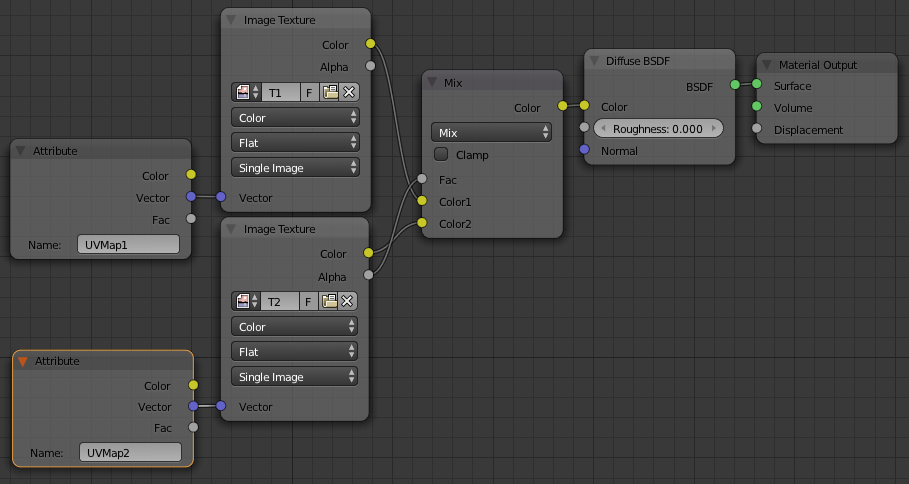
\includegraphics[width=\textwidth]{resources/Blender.png}
  \caption{Blender's node-based interface}
  \label{fig:blender}
\end{figure}

Unlike data processing languages, Blender's node base interface isn't used to handle stream data but instead is a replacement for list-like user interfaces in previous versions. Blender allows to group nodes into subnodes, allowing the abstraction of complex functionality into a single interface element.

\subsubsection*{Discussion}
The strengths of dataflow programming lie in the concept of configurable modularity, allowing for the same black-box components to be used multiple times. Additionally, some implementations also allow grouping multiple nodes into subnodes, leading to a very high level of abstraction. This also leads to great maintainability, an area often disregarded in literature, despite the fact that companies usually spend a high amount of their resources on application maintenance. Furthermore, applications designed on the dataflow paradigm display an impressive robustness while being surprisingly performant especially in a massively parallel setting. When implemented as a visual programming language, dataflow programming also exploits the developer's visual cognitive skills, and allows for incremental software development and maintenance. The focus on the flow of data between components rather than the functionality of the components themselves introduces a natural notion of user-configurable control flow, further contributing to the flexibility and expressiveness of the model.

\section{Research Question}
\label{sec:res_question}
The background knowledge about dataflow programming and visual query builders established in Section~\ref{sec:background} suggests that the motivating idea of creating a visual query builder based on dataflow programming is viable. Some related work, particularly DFQL, can be seen as proof, that dataflow programming can be used to create queries on the relational model. This thesis will examine whether it is also suitable to create a tool that produces SQL code. The focus lies on creating a tool as powerful as possible, covering all major features of SQL while ensuring correctness of the resulting query whenever possible. Furthermore, it should feature a highly visual and easy to use interface based on dataflow programming. In short, the thesis will therefore answer the following question:

How can the dataflow programming paradigm be leveraged to create a powerful, yet easy to use visual SQL query builder?

\section{Method}
To answer the research question, we will first compile the list of features a powerful query builder needs to support. Based on these requirements, we then develop the theoretical specification and a proof-of-concept implementation of a query builder we call QENoBI, which is an acronym for \textbf{Q}uery \textbf{E}ngineering on a \textbf{No}de-\textbf{B}ased \textbf{I}nterface.

%---------------
%Approach
%---------------

\chapter{Approach}
\label{ch:approach}

\section{Requirements}
\label{sec:requirements}
This chapter discusses the theoretical specification of QENoBI, starting with the list of requirements based on the analysis of a test set of queries. Specifically, we will compile a list of all the features that are necessary to achieve a high coverage of SQL along with a high level of usability.

\subsection{Test Set}
\label{sec:test_set}
In order to accurately establish the requirements for a general-purpose SQL query builder, we compile a set of queries covering the most commonly used features of SQL. This approach is chosen due to the fact that starting directly from the SQL specification is infeasible due to its scope and inconsistencies between vendors. An unbiased test set on the other hand puts the focus on actual real-life demands, covering only the most commonly used features. To meet these requirements, the set was mostly assembled from queries taken from open-source applications. This turned out to be somewhat more involved than expected, as most larger applications make use of object-relational mapping libraries such as Hibernate, JDBC or Ruby on Rails. Therefore, queries are often not available in plain text and would have to be translated manually, which often results in overcomplicated and therefore unrepresentative queries. An overview of the test set is presented in Table~\ref{tab:test_set} while the actual queries can be found in the appendix. It consists of 20 queries from 6 different sources. The queries are written for a number of different DBMS specifically MySQL, Oracle and Microsoft SQL Server. Additionally, the queries from the book ``Database Management Systems''\cite{ramakrishnan2000dms} are DBMS independent due to their low complexity.

\begin{table}[h!]
\centering
\begin{tabu} to \textwidth {l c c}
\toprule
\textbf{Source}								& \textbf{Complexity}	& \textbf{Quantity}	\\
\midrule
Database Management Systems					& low					& 9					\\
Wikipedia									& varies				& 2					\\
Typo3										& medium				& 2					\\
Joomla										& medium				& 1					\\
LedgerSMB									& varies				& 4					\\
Microsoft Benchmark							& high					& 2					\\
\bottomrule
\end{tabu}
\caption{Test Set}
\label{tab:test_set}
\end{table}

The test set can be used to reveal strengths and weaknesses in the query builders discussed in Section~\ref{sec:vis_qb} and, in part, to evaluate the performance of QENoBI. Furthermore, since the queries represent a relatively unbiased selection, they can be used to assess the relevancy of certain features by comparing their relative frequency. Specifically, if a feature is present in a large number of the queries, it will have a strong negative impact on the test results of a query builder that doesn't support the feature. Vice versa, a query builder that supports the feature will receive better test results, indicating that it is based on a beneficial architecture. Therefore, common features have a stronger impact on the test results.

\subsection{Features}
\label{sec:feature_set}
In order to be both powerful and easy to use, a query builder must satisfy a number of features, which can be separated into three categories:

\begin{description}
\item[Relational Algebra] containing the operators of the relational algebra, such as different the types of joins, selection and projection.

\item[SQL Features] containing additional features of SQL that are not part of the relational algebra, such as sorting.

\item[UI \& Usability] containing features that improve the overall usability, particularly for novice users, as well as characteristics of the graphical user interface.
\end{description}

The features of the first category are extracted directly from the definition of the relational algebra while the second category is based on the analysis of the test set. Since SQL implementations differ significantly between vendors, the features in the second category are relatively high level, focussing on semantic rather than syntactic constructs. For instance, while the syntax to limit the number of entries in the result set varies greatly, the feature itself is present in all major implementations. Since the features in these two categories represent elements of the specification of either the relational algebra or SQL, they directly influence the SQL coverage of the query builder. This is in contrast to features from the last category, which, from an coverage point of view, are non-essential. However, since the key purpose of query builders is to simplify the construction of queries, providing a high level of usability and a powerful user interface is just as important as achieving a high SQL coverage. To reinforce that point, consider the extreme example of a query builder that consists of a single text area that automatically highlights keywords. Clearly, this represents the most powerful query builder possible in terms of coverage, however, the improvements in usability are so minimal that the practical use of the tool is essentially non-existent. The usability features were collected by analyzing existing query builders and concepts using queries from the test set and are therefore somewhat subjective. The list of requirements is presented in Table~\ref{tab:features}.
\begin{table}[h!]
\centering
\begin{tabu} to 0.85\textwidth {X[l] X[l] X[l]}
\toprule
\textbf{Relational Alg.}	& \textbf{SQL Features}	& \textbf{UI \& Usability}	\\
\midrule
Projection					& Expressions			& Visual					\\
Selection					& Sort					& Abstraction				\\
Rename						& Limit					& Contextual				\\
Natural Join				& Distinct				& Correctness				\\
$\theta$-Join				&						& Readability				\\
Outer Join					&						& 							\\
Semi/Anti-Join				&						&							\\
Aggregation					&						&							\\
Subqueries					&						&							\\
Set Operations				&						&							\\
\bottomrule
\end{tabu}
\caption{List of features}
\label{tab:features}
\end{table}

Some of the features in this list, particularly the ones in the usability category, are somewhat non-descriptive and are therefore be explained below.
\begin{description}
\item[Visual] Does the query builder feature a visual user interface?
\item[Abstraction] Does the user have to understand SQL to write a query?
\item[Contextual] Does the builder use available information, e.g. is it type-aware?
\item[Correctness] Are the generated queries syntactically and semantically correct?
\item[Readability] Are the generated queries human-readable?
\end{description}
Note that optimization of the queries is not part of this list. This is due to the fact that performance varies greatly between vendors and is therefore difficult to assess without large scale testing. Furthermore, database vendors invest tremendous efforts on query optimizers, meaning that queries will most likely result in the same execution plans regardless of whether they are optimized or not. Moreover, the focus of this thesis is on the visual aspect of the builder rather than on the performance aspect.

The list of features can now be employed to reveal and understand the limitations of existing query builders by evaluating, for every feature, whether it is fully, partially or not at all supported by the query builders. For features that are not supported, we also assess whether this limitation is inherent to the design or is simply a missing feature that could be implemented without significantly changing the user interface or the underlying architecture. From the results of this evaluation, we should be able to narrow down the most important areas that need to be covered in the specification. Furthermore, design choices and the impacts of these choices on the query builders will deliver valuable insights that will help in the design phase later on. The three query builders tested are the examples from Section~\ref{sec:vis_qb}, EasyQuery, ExtJS and DFQL. All three are based on different interface concepts, leading to substantial differences in the test results listed in Table~\ref{tab:eval}.
\begin{table}[h!]
\centering
\begin{tabu} to 0.85\textwidth {l X[c] X[c] X[c]}
\toprule
							& EasyQuery			& ExtJS				& DFQL				\\
\midrule
\textbf{Relational Algebra}	&					&					&					\\
Projection					& \tc{g}{yes}		& \tc{o}{partial}	& \tc{g}{yes}		\\
Selection					& \tc{g}{yes}		& \tc{g}{yes}		& \tc{g}{yes}		\\
Rename						& \tc{g}{yes}		& \tc{g}{yes}		& \tc{g}{yes}		\\
Natural Join				& \tc{o}{implicit}	& \tc{r}{no}		& \tc{o}{possible}	\\
$\theta$-Join				& \tc{o}{implicit}	& \tc{o}{partial}	& \tc{g}{yes}		\\
Outer Join					& \tc{o}{implicit}	& \tc{g}{yes}		& \tc{o}{possible}	\\
Semi/Anti-Join				& \tc{r}{no}		& \tc{r}{no}		& \tc{o}{possible}	\\
Aggregation					& \tc{g}{yes}		& \tc{g}{yes}		& \tc{g}{yes}		\\
Subqueries					& \tc{o}{partial}	& \tc{r}{no}		& \tc{g}{yes}		\\
Set Operations				& \tc{r}{no}		& \tc{r}{no}		& \tc{g}{yes}		\\
\midrule
\textbf{SQL Features}		&					&					&					\\
Expressions					& \tc{r}{no}		& \tc{g}{yes}		& \tc{g}{yes}		\\
Sort						& \tc{g}{yes}		& \tc{g}{yes}		& \tc{g}{yes}		\\
Limit						& \tc{r}{no}		& \tc{r}{no}		& \tc{o}{possible}	\\
Distinct					& \tc{r}{no}		& \tc{r}{no}		& \tc{i}{}			\\
\midrule
\textbf{Usability}			&					&					&					\\
Visual						& \tc{r}{low}		& \tc{o}{medium}	& \tc{g}{high}		\\
Abstraction					& \tc{o}{medium}	& \tc{r}{low}		& \tc{g}{high}		\\
Contextual					& \tc{g}{high}		& \tc{r}{low}		& \tc{r}{low}		\\
Correctness					& \tc{g}{high}		& \tc{r}{low}		& \tc{r}{low}		\\
Readability					& \tc{o}{medium}	& \tc{g}{high}		& \tc{i}{}			\\
\bottomrule
\end{tabu}
\caption{Evaluation of the query builders}
\label{tab:eval}
\end{table}
Green boxes indicate a positive test result, e.g. that the feature is fully implemented, while red boxes indicate the opposite, e.g. features that are not present at all or only in a very limited fashion. Finally, orange boxes indicate features that are only partially supported. Feature that are not implemented but could be added in a very straightforward way are also indicated by orange boxes. Since DFQL is not an SQL query builders, the readability of its output cannot be compared and is indicated by a gray box. Similarly, the \texttt{DISTINCT} feature of SQL has no counterpart in DFQL, as it operates on the relational model.

In order to learn from the designs we studied, we need to analyze what characteristic of a query builder enables it to meet a certain requirement. 
As a consequence, the most interesting features are the ones, where some query builders outperform the others. If a feature is present in all three query builders, then we assume that it can be implemented regardless of approach. Conversely, if a feature is not implemented in any of the query builders, we assume that it is tricky, regardless of approach. Those features will have to be addressed independently, as there is no previous work to refer to.

DFQL significantly outperforms the other query builders in the first category. For the most part, it owes this to its dataflow based architecture. For instance, while DFQL implements neither the semi- nor the anti-join, both could be added with minimal effort by simply adding two new nodes that cover those features. EasyQuery on the other cannot be extended in the same manner, as it handles joins implicitly. Similarly, ExtJS cannot be extended to support the feature, as joins are created by connecting two columns, creating the join condition for a $\theta$-join. Unlike the other two query builders, ExtJS does not allow for the same column to be projected multiple times. While one could argue that this feature is very rarely used, it is essential for a large number of reasonable queries. For instance, it is required to construct the query in Listing~\ref{lst:multiple_agg} which retrieves the maximum, minimum and average of a certain column.
\begin{codeex}[caption=A query that uses the same column multiple times, label=lst:multiple_agg]
SELECT MAX(age), MIN(age), AVG(age)
FROM Sailors;
\end{codeex}

The query in Listing~\ref{lst:multiple_agg} operates on the Sailors schema borrowed from the book ``Database Management Systems'' by Raghu Ramakrishnan and Johannes Gehrke\cite{ramakrishnan2000dms}. We will use this schema extensively to examine example queries. The schema consists of the following three tables:
\begin{description}
\item[Sailors](sid, sname, age, rating)
\item[Boats](bid, bname, color)
\item[Reserves](sid, bid, day)
\end{description}

Finally, two major differences in this category are found in the last two features. Once again, DFQL outperforms both EasyQuery and ExtJS by featuring full and arbitrarily deep subquery support as well as set operations. Both features are possible due to certain characteristics of dataflow programming that will be discussed in more detail in Section~\ref{sec:pow_df}. For now, it suffices to say that the concepts used by EasyQuery and ExtJS are static in term of control flow, fixed on a single query. Dataflow programming on the other hand introduces input dependencies (i.e. subqueries) and therefore supports user-defined control flow.

The second category is interesting, in that no query builder manages to achieve a satisfying coverage. Despite limiting itself to the relational algebra, DFQL offers additional features such as sorting and while it is not implemented as a primitive, a means to limit the number of output rows could be easily added as well. Both features, sort and limit, are not part of the relational algebra, which is based on sets that are unordered by definition. For the same reasons, all rows in DFQL are distinct by definition, eliminating the need for a distinct modifier. ExtJS does not support \texttt{LIMIT} or \texttt{DISTINCT}, but features sorting as well as arbitrarily complex expressions. This sets it apart from EasyQuery which does not support expressions. However, the feature is completely text based which has severe consequences on the usability of the tool. Furthermore, enforcing correctness on textual input is quite costly and might not be possible at all in certain cases.

Similar to the previous category, the results from the usability category reveal significant differences between the three tools. DFQL features a highly visual interface that covers most of its functionality while the visual part of ExtJS is limited to creating joins. As mentioned in the introduction, EasyQuery's interface has no visual elements at all, relying on a list based approach instead. In order to simplify query construction for novice users, a visual query builder should abstract SQL into a more consistent form. For instance, SQL requires that constraints on aggregates are placed in the \texttt{HAVING} clause as opposed to the \texttt{WHERE} clause. While this makes perfect sense from a technical point of view and is no issue to the experienced SQL user, novice users will likely find this behavior confusing. Therefore, it makes sense to abstract both types of constraints into a single construct. This particular problem is not addressed by any of the query builders, as neither ExtJS nor EasyQuery support conditions on aggregates and DFQL, being based on the relational algebra, never encounters the issue in the first place. In order to remove complexity, EasyQuery introduces the implicit join, based on an extended database schema. This works reasonably well but makes it impossible to construct cetain queries, e.g. queries that contain a self-join or a join that is not based on foreign keys. Since the relational algebra is a mathematical concept and not a programming language, it is both concise and consistent. As DFQL merely provides primitives for a number of operators from the relation algebra, in inherits these properties. Combined with dataflow programming, this naturally leads to a very clean and uniform interface based on the simple concept of the node. Moreover, DFQL offers the ability to create subnodes, allowing the creation of new operators by combining primitives or other subnodes. This configurability makes DFQL highly abstract and sutiable for novice users as well as experts. Specifically, novice users can take advantage of subnodes due to their increased abstraction while expert users can group frequently used queries into a subnode, resulting in more efficient query construction. Subnodes are discussed extensively in Section~\ref{sec:subnodes}.

The key feature that sets EasyQuery apart from the DFQL and ExtJS is that it is highly contextual, using types and even table contents to limit the available options and provide hints to the user. For instance, EasyQuery adjusts the available comparison operators to the type of the column. Furthermore, aside from a few special cases, EasyQuery always produces syntactically correct queries. These two features are extremely valuable from a usability point of view as they greatly simplify query construction by providing hints to novice users, who are unable to understand and therefore manually debug the output. Neither of these two features are found in any of the other query builders. This is somewhat surprising, since support for the feature is not inherent to EasyQuery's architecture, and could therefore be implemented on the other tools as well. That being said, EasyQuery makes a number of compromises to simplify ensuring query correctness. Specifically, expressions based on textual input are difficult to check as discussed on multiple occasions and are therefore lacking. While DFQL provides by far the most visual interface, many of its inputs, such as the join condition or the list of projected columns, are still text-based, therefore not making use of any contextual information.

In order to provide the best possible user experience, a query builder should output readable, concise  SQL queries. This is not the case with EasyQuery, which doesn't use the star notation and instead defaults to projecting every column explicitly. Moreover, it automatically assigns an alias to every column, leading to massive \texttt{SELECT} statements. This is loosely related to correctness concerns that are covered in Section~\ref{sec:aliasing}. Note that one could argue in favor of this behavior by noting that the list of projected columns is known without knowledge of the schema. One the other hand, the star notation guarantees, that all columns of a table are projected, again without knowledge of the schema. Therefore, both strategies have their advantages but clearly cannot be combined and we consequently choose the one that results in shorter queries. For comparison, queries produced by ExtJS are a lot more readable, which, ironically, is due to the fact that ExtJS doesn't spend any efforts processing the inputs. Listings~\ref{lst:read_easyquery} and \ref{lst:read_extjs} compare the same query generated by EasyQuery and ExtJS respectively. Finally, DFQL is meant as a replacement for SQL and consequently doesn't output any SQL code.

\begin{codeex}[caption=``Bloated'' query generated by EasyQuery, label=lst:read_easyquery]
SELECT Cust.[CompanyName] AS [Customer Company name],
  Cust.ContactName AS [Customer Contact name],
  Cust.ContactTitle AS [Customer Contact title],
  Cust.Address AS [Customer Company address],
  Cust.Country AS [Customer Country],
  Cust.City AS [Customer City],
  Cust.Fax AS [Customer Fax],
  Cust.Phone AS [Customer Phone],
  Cust.PostalCode AS [Customer Postal Code],
  Cust.Region AS [Customer Region] 
\end{codeex}
\begin{codeex}[caption=Concise query generated by ExtJS, label=lst:read_extjs]
SELECT *
FROM Customers
\end{codeex}
FROM Customers AS Cust

\subsection{Discussion}
A quick glance at the results suggests that DFQL is more powerful than the other two query builders tested, and the feature-by-feature analysis delivers a significant amount of evidence to support this impression. DFQL not only provides a highly abstract and customizable interface but also manages to achieve the highest SQL coverage. While it has a number of limitations, mostly originating from its relatively heavy use of text-based inputs, these are not inherent the dataflow approach. Overall, the dataflow programming paradigm appears to be remarkably well suited to implement a visual SQL query builder.

\section{Concepts}
\label{sec:concepts}
In this section, we will discuss some of the things we learned from the analysis in Section~\ref{sec:feature_set} and how they influence the design of QENoBI. Specifically, we will study a number of correlations found in the test results and their implication on the design process.

\subsection{Power and Dataflow}
\label{sec:pow_df}
Traditional imperative languages model programs as a series of sequentially executed operations. Control flow is handled by means of conditional statements, based on the current state of the execution. Dataflow programming on the other hand focuses on the movement of data, treating functions as black boxes that are executed once all its inputs are available. Therefore, a natural way to illustrate dataflow programs is to use graphs, where the nodes denote functions and the edges denote flow of data, connecting outputs of one node to inputs of another. While SQL was designed to be as similar to natural language as possible, graph representations are widely used to illustrate queries on the relational model. Figure~\ref{fig:rel_alg_graph} shows a query on the relational model represented as a graph.

\begin{figure}[h]
  \centering
  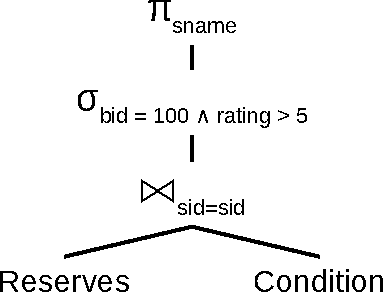
\includegraphics[width=0.4\textwidth]{resources/RelAlgGraph.pdf}
  \caption{A query on the relational model illustrated as a graph}
  \label{fig:rel_alg_graph}
\end{figure}

The reason this works particularly well, is that the relational model is based on an algebra and therefore adheres to the group axioms. Specifically, it satisfies the requirement of operational closure, meaning that the result of any operation on relations is again a relation. This is extremely beneficial when looking at graph-based languages, as it means that any output produced can be used as an input to any other node. With respect to database queries, this provides a very natural representation of nested queries, which is one of the most noted weaknesses of SQL. This also explains, how DFQL manages to perform so much better than query builders based on a more static approach. While DFQL only targets the relational algebra, we can assume that the benefits will also apply to a query builder covering a large part of all SQL statements.

\subsection{Power and Correctness}
The discussion of the test results in Section~\ref{sec:feature_set} hinted at a negative correlation between the power of a query builder and its ability to produce correct queries. In other words, it appears that ensuring query correctness comes at the cost of significantly reduced power, as is the case with EasyQuery. This makes sense intuitively, as allowing a large number of queries to be constructed means that more cases need to be covered. For instance, supporting subqueries requires a very modular system capable of proving correctness for arbitrarily deep subquery chains. While ExtJS and DFQL support expressions, they both do so based on text-based inputs, sacrificing the ability to easily validate the correctness of the query. Therefore, in order to ensure that generated queries can be shown to be syntactically correct, QENoBI should not rely on text-based input whenever possible.

\subsection{Dataflow and Abstraction}
One of the major strengths of dataflow programming is the concept of subnodes, essentially allowing the creation of new operators from primitives and other subnodes. In the case of DFQL, this results in a highly customizable and abstract interface.

\section{Design}
\label{sec:design}
The design process is separated into multiple stages. We start out by deciding on an architecture and then from that derive the list of nodes. As a next step, we discuss the functionality of the nodes one by one and finally cover some of the usability topics.

\subsection{Architecture}
\label{sec:arch}
As discussed in Section~\ref{sec:dfp}, dataflow programs can be represented as graphs, where nodes represent functions that exchange data across the edges. In the context of databases, the data could for instance be relations, columns or conditions. We will explore and compare two different approaches, the first being based on columns, the second being based on relations as their working units. Since the query is based on a graph, it is built piece by piece, it exists in multiple stages, meaning that there are multiple possible queries that could be generated. In fact, in the second approach, any output produced by a node is a valid query. Both approaches therefore rely on an output node that translated and outputs the query connected to its input.

The core idea of the column based approach is based on a table node that exposes all the columns of the relation, which can then be used directly to for instance add constraints or aggregate a certain column. Additionally, with the focus being on columns, projecting a column is achieved by simply connecting a column to the output node. This works quite well for simple queries such as the one illustrated in Figure~\ref{fig:col_agg} which aggregates and projects a single column.

\begin{figure}[h]
\begin{codeex}
SELECT MAX(rating)
FROM Sailors
\end{codeex}

  \centering
  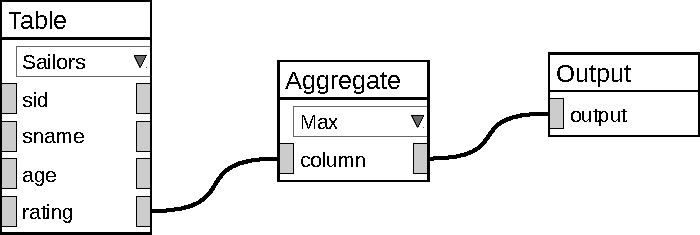
\includegraphics[width=0.8\textwidth]{resources/ColAgg.pdf}
  \caption{Simple query on column based approach}
  \label{fig:col_agg}
\end{figure}

In the column based approach, most operations are implemented using the idea of pattern matching. In addition to the output, each column also has an input that can be used to constrain the values of the column. For instance, a query that returns all the ratings of sailors named `Bob' is shown in Figure~\ref{fig:col_patmat}.

\begin{figure}[h]
\begin{codeex}
SELECT rating
FROM Sailors
WHERE sname = 'Bob'
\end{codeex}

  \centering
  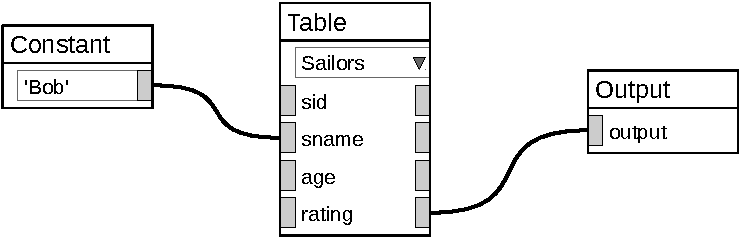
\includegraphics[width=0.8\textwidth]{resources/ColPatMat.pdf}
  \caption{Pattern matching in the column based approach}
  \label{fig:col_patmat}
\end{figure}

Note that there is no limitation on the number of inputs. If multiple constraints are attached to input, all of them need to be met in order for a row to remain in the result set. For instance, to constraint the rating column to numbers between 5 and 10, we introduce a comparison node that takes a comparison operator and a constant and attach two of those, $\leq$ 10 and $\geq$ 5, to the input of the rating column. Lists, including columns, can also be used as patterns as well, which are satisfied if the value occurs in the list. As such, list patterns are a simple implementation of SQL's IN-construct.

Overall, the pattern matching approach appears to work well for very simple queries but has a number of serious shortcomings. While list patterns can be used to emulate certain join types (specifically a semi-join on a single column), they cannot modify the layout of a table, i.e. add or remove columns and as such are unsuited to model the behavior of a $\theta$- or natural join. This is caused by the fact that the column approach essentially splits relations into single columns and then treats them independently. Therefore, an additional construct would have to be introduced to temporarily merge multiple columns into a relation. Likewise, constraints on multiple columns, such as finding all sailors with a rating that exceeds their age, are impossible to describe using this approach. There are numerous other features that exhibit similar problems, which could only be resolved by adding additional nodes, resulting in a two class system, where multiple ways can be used implement the same functionality. From a usability point of view, this is highly unfavorable and should be avoided, as it is likely to confuse novice and expert users alike. Ultimately, a different, more uniform approach is required.

The second approach is based on relations and conceptually very similar to list processing in functional languages such as Haskell. It can be considered an extension of the relational algebra and inherits many of its beneficial characteristics, one of these being operational closure which was discussed in Section~\ref{sec:pow_df}. The core idea of the architecture is to shape the query in an interactive manner, with each node modifying the relation in a specific way. This approach is closer to the assembly line metaphor introduced in Section~\ref{sec:dfp} which models queries as assembly lines that move data from worker to worker transforming it one step at a time. This works very well in concept, as relations can be understood as a list of tuples. For instance, a constraint on an column, like the one used in the query in Figure~\ref{fig:col_patmat} could be implemented in Haskell using the filter function, which takes a list and a predicate and returns a new list consisting of all the tuples that satisfy the predicate. The same query implemented using the relation based approach is depicted in Figure~\ref{fig:rel_constraint}.

\begin{figure}[h]
\begin{codeex}
SELECT *
FROM Sailors
WHERE sname = 'Bob'
\end{codeex}

  \centering
  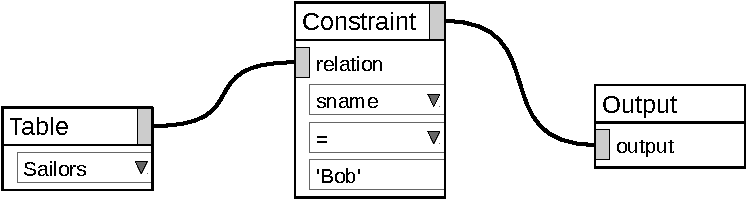
\includegraphics[width=0.8\textwidth]{resources/RelConstraint.pdf}
  \caption{Selection in relation based approach}
  \label{fig:rel_constraint}
\end{figure}

Note that since the data passed across the connection is a relation, it is now necessary, to declare what column is supposed to be constrained. In general, the approach feels somewhat less elegant than the pattern matching approach but can handle column-column constraints. Due to the strong similarities between this architecture and the relational algebra, all relational operators can be translated directly. While this greatly simplifies the design process, it comes at the risk of remaining too conservative, resulting in a tool that does not represent a significant improvement over SQL.

An interesting aspect of the relation-based approach is that the progressive construction of the query models the execution of the query on the database. To support this intuition, a tool could in theory offer the possibility to inspect intermediate results, which could be tremendously helpful in debugging a query that doesn't return the expected results. DFQL actually implements this by allowing multiple DISPLAY nodes that can be attached at any point in the query. In the case of DFQL, these intermediate results are easy to obtain, since DFQL is not a query builder relying on a DBMS but actually executes the queries on its own. An pure SQL query builder could still emulate this behavior by running the intermediate queries. However, depending on the DBMS used and of course the query, this process could be very expensive, as the DBMS will most likely run the same queries multiple times. Additionally, it might use different execution plans for partial queries, potentially resulting in inaccuracies. Nonetheless, it could be a very useful feature and again underlines the advantages of dataflow based query builders. To circumvent these issues, an SQL query builder could simply output the partial query instead of the results.

\subsection{Nodes}
\label{sec:nodes}
To get started, we compile a list of the nodes that we assume are necessary to cover most of the features in Table~\ref{tab:features}. Since this list of features is derived from the definitions of the relational algebra as well as SQL, most features will directly translate into their own node. Some straightforward simplifications, such as merging all join types into one node, will be applied without discussion. The list is presented in Table~\ref{tab:nodes_assumption}. The names of the nodes are chosen to be more intuitive than the terminology used in SQL or the relational algebra.
\begin{table}[h!]
\centering
\begin{tabu} to 0.65\textwidth {X[l] X[l]}
\toprule
\textbf{Node}		& \textbf{Functionality}	\\
\midrule
Table				& Relation					\\
Output				& Output					\\
Constraint			& Selection (Filter)		\\
Join				& Joins						\\
Select				& Projection				\\
Aggregate			& Aggregation				\\
Distinct			& Distinct					\\
Rename				& Alias (Column)			\\
Merge				& Set Operations			\\
Expression			& Expressions				\\
Constant			& List of constants			\\
Sort				& Sorting					\\
Limit				& Limiting					\\
\bottomrule
\end{tabu}
\caption{List of Nodes}
\label{tab:nodes_assumption}
\end{table}\\
As mentioned before, this list is based on the assumption that the list of features translates directly into the list of nodes. However, the discussion of the functionality of some of the nodes will reveal that this assumption does not hold in for all nodes leading to changes in the list.

\subsubsection*{Table}
\begin{wrapfigure}{l}{0.23\textwidth}
  \vspace{-13pt}
  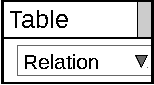
\includegraphics[width=0.2\textwidth]{resources/Table.pdf}
  \vspace{-5pt}
\end{wrapfigure}
The Table node is one of the most basic nodes. It serves as the source of all the data in a query and as such doesn't have any inputs. The desired relation can be selected from a drop-down list.
\wrapfill

\subsubsection*{Output}
\begin{wrapfigure}{l}{0.23\textwidth}
  \vspace{-13pt}
  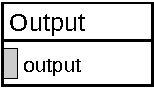
\includegraphics[width=0.2\textwidth]{resources/Output.pdf}
  \vspace{-5pt}
\end{wrapfigure}
The Output node serves as the ``drain'' of the query and is the only node without an output. Due to its unique role, it is also the only node that cannot be deleted and the only node present in a new, otherwise empty query.

\subsubsection*{Constraint}
\begin{wrapfigure}{l}{0.23\textwidth}
  \vspace{-13pt}
  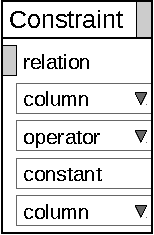
\includegraphics[width=0.2\textwidth]{resources/ConstraintBasic.pdf}
  \vspace{-5pt}
\end{wrapfigure}
The Constraint node is used to remove rows from a relation that do not satisfy a certain predicate. Metaphorically speaking, it is a worker that filters all the rows with respect to the predicate. The SQL equivalent is the WHERE statement.\\
In DFQL, the predicate is supplied in text form. This represents a very flexible approach, as it allows arbitrarily complex expressions, but makes it difficult to ensure correctness. Furthermore, the user needs to be familiar with the syntax of the expressions, imposing difficulties for novice users. Therefore, we want to take a more user-friendly approach, by providing a fixed user interface that takes a column and compares it to a constant or alternatively to another column. This approach also simplifies correctness evaluations, which are discussed in Section~\ref{sec:correctness}.

\subsubsection*{Join}
\begin{wrapfigure}{l}{0.23\textwidth}
  \vspace{-13pt}
  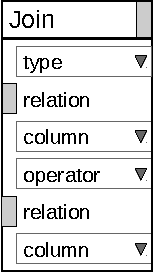
\includegraphics[width=0.2\textwidth]{resources/Join.pdf}
\end{wrapfigure}
The Join node, as the name suggests, handles all different types of joins. A drop-down list is used to indicate the type of the join. Depending on the type chosen, the node will change appearance, providing all the necessary inputs. A natural join for instance only requires two relations and the same holds for the semi- and anti-join. The $\theta$-join on the other hand additionally requires a join condition. Therefore, the interface is expands, allowing the user to define a column to column comparison. The extended state, shown to the left, strongly resembles the constraint node. Furthermore, this representation does not allow complex join conditions but is instead limited to a single comparison. Both facts will be addressed in Section~\ref{sec:issues}.
\wrapfill

\subsubsection*{Select}
\begin{wrapfigure}{l}{0.23\textwidth}
  \vspace{-13pt}
  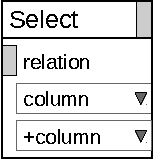
\includegraphics[width=0.2\textwidth]{resources/Select.pdf}
  \vspace{-5pt}
\end{wrapfigure}
The Select node is named after the SQL select statement and not the relational algebra operator and therefore represents a projection. Most query builders implement projection by providing a list displaying a checkbox for every column of the relation. This is approach is arguably intuitive but problematic, as it doesn't allow projecting the same column more than once. Also, reordering of the columns is impossible, a feature that is especially important in conjunction with set operators, as they require type-identical table layouts. Due to these reasons, we examine a different, more flexible approach, featuring a dynamic column list. The user can attach a relation and then select a column from a drop-down list. Once a column is selected, another row is automatically added, meaning that an arbitrary number of columns can be selected.
\newpage

\subsubsection*{Aggregate}
\begin{wrapfigure}{l}{0.23\textwidth}
  \vspace{-13pt}
  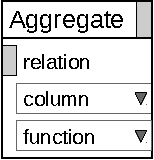
\includegraphics[width=0.2\textwidth]{resources/Aggregate.pdf}
  \vspace{-5pt}
\end{wrapfigure}
The Aggregate node is relatively straightforward, allowing the selection of a column and aggregate function. However, it turns out that an implementation like this does not work in practice, since different behaviors might be expected depending on the type of query. Specifically, it is unclear whether the aggregation should replace the original column or not. This problem will be addressed in Section~\ref{sec:issues}.
\wrapfill

\subsubsection*{Distinct}
\begin{wrapfigure}{l}{0.23\textwidth}
  \vspace{-13pt}
  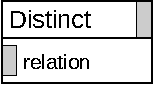
\includegraphics[width=0.2\textwidth]{resources/Distinct.pdf}
  \vspace{-5pt}
\end{wrapfigure}
The Distinct node removes all duplicates in a relation and therefore requires only a very simple interface.
\wrapfill
\vspace{30pt}

\subsubsection*{Rename}
\begin{wrapfigure}{l}{0.23\textwidth}
  \vspace{-13pt}
  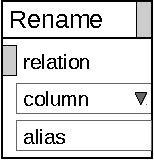
\includegraphics[width=0.2\textwidth]{resources/Rename.pdf}
  \vspace{-5pt}
\end{wrapfigure}
The Rename node can be used to assign aliases to columns. The structure of the node is similar to the aggregation node, featuring a relation, column drop-down list and a text field to set the alias. Renaming is a somewhat problematic feature, due the fact that the column name must be unique. As a consequence, if two tables are joined that contain an equally named column, one of them is dropped. We will also discuss this in Section~\ref{sec:issues}.
\wrapfill
\vspace{-5pt}

\subsubsection*{Merge}
\begin{wrapfigure}{l}{0.23\textwidth}
  \vspace{-13pt}
  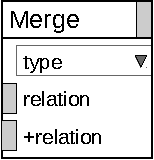
\includegraphics[width=0.2\textwidth]{resources/Merge.pdf}
  \vspace{-5pt}
\end{wrapfigure}
The Merge node implements the set operators. Its interface works similarly to the projection in that it contains a dynamic list, taking an arbitrary number of relations. Set operations have special typing requirements on the columns of the relations. Therefore, they will be revisited in the section on correctness.
\wrapfill
\vspace{32pt}

\subsubsection*{Expression}
\begin{wrapfigure}{l}{0.23\textwidth}
  \vspace{-13pt}
  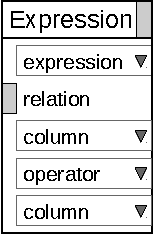
\includegraphics[width=0.2\textwidth]{resources/Expression.pdf}
  \vspace{-5pt}
\end{wrapfigure}
Due to the differences in dialects, the interface of the Expression node has to be completely dynamic. The structure shown to the left is tailored to allow arithmetic-like operations, for instance adding a constant to an integer column or a prefix to a text column. Other expressions such as acquiring the current system date, don't take any parameters while others might take many more. Additionally, expressions differ significantly between database vendors, meaning that the expressions would either have to be customizable or limited to a specific dialect.
\wrapfill

\subsubsection*{Constant}
\begin{wrapfigure}{l}{0.23\textwidth}
  \vspace{-13pt}
  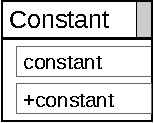
\includegraphics[width=0.2\textwidth]{resources/Constant.pdf}
  \vspace{-5pt}
\end{wrapfigure}
The Constant node features a very simple interface consisting of an arbitrary number of text fields. The key purpose of this node is to create lists of constants that can be used in \texttt{IN} expressions. Internally, its output is handled as a relation with a single column.
\wrapfill
\vspace{20pt}

\subsubsection*{Sort}
\begin{wrapfigure}{l}{0.23\textwidth}
  \vspace{-13pt}
  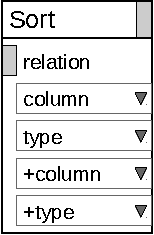
\includegraphics[width=0.2\textwidth]{resources/Sort.pdf}
  \vspace{-5pt}
\end{wrapfigure}
The Sorting node supports an arbitrary number of sorting columns and as such requires a slightly more elaborate interface. The interface takes an arbitrary number of pairs of columns and sort types. Whenever a column is selected, a new one is appended to the list.
\wrapfill
\vspace{80pt}

\subsubsection*{Limit}
\begin{wrapfigure}{l}{0.23\textwidth}
  \vspace{-13pt}
  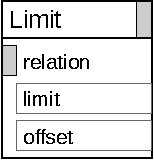
\includegraphics[width=0.2\textwidth]{resources/Limit.pdf}
  \vspace{-5pt}
\end{wrapfigure}
Finally, the Limit node is very minimalistic and straightforward, taking only three parameters, a relation and two positive integer. The integer parameters define the number of rows to fetched and the offset. The interface is modeled after the PostqreSQL implementation of \texttt{LIMIT} but could produce code for any dialect.
\wrapfill
\vspace{60pt}

\subsection{Issues and Refinements}
\label{sec:issues}
This section discusses the various issues that became apparent in the Section~\ref{sec:nodes}. We will address these issues by determining their root cause and then finding a way to resolve them. For reference, we will also examine how DFQL deals with these issues.

\subsubsection*{Logical Connectives}
The assembly line metaphor works very well to illustrate the functionality of dataflow programs. Therefore, it can also be used to illustrate some of the weaknesses of the approach taken here. One major issue of the system arises from the fact that if a certain row fails to satisfy a constraint, the row is permanently removed. This, combined with the fact that the constraint node only allows the declaration of a single expression, means that disjunctions, OR statements in SQL, cannot be implemented at all. For instance, given predicates $P$ and $Q$, and a row $x$ in relation $T$ where $P(x)$ and $\neg~Q(x)$ hold, the composite predicate $P(x)~\vee~Q(x)$ cannot be properly expressed. If $Q$ is checked before $P$, x will be dropped and can't be recovered later on, because it is no longer in the relation. Likewise, a row $y$ with $\neg~P(y)$ and $Q(y)$ would be dropped if the order is reversed. The only way disjunction can be implemented correctly in this approach is by splitting the base relation output, applying the constraints independently and then combining the results. This approach is illustrated in Figure~\ref{fig:disjunction}.

\begin{figure}[h]
  \centering
  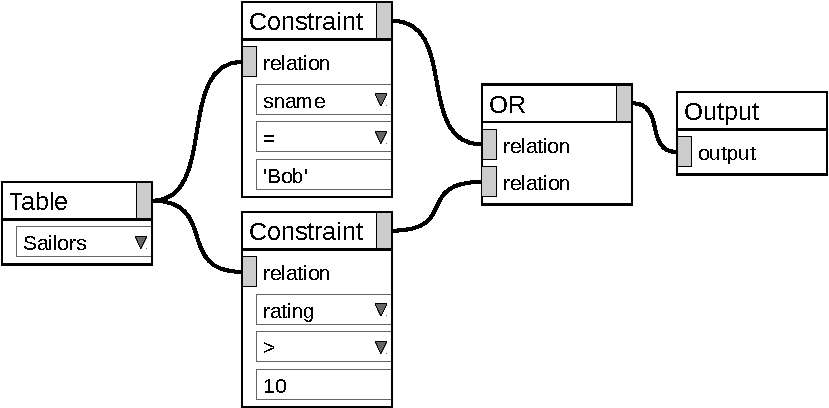
\includegraphics[width=0.9\textwidth]{resources/Disjunction.pdf}
  \caption{Disjunction by splitting and merging the relation}
  \label{fig:disjunction}
\end{figure}

The OR node used in this example is not defined yet. However, it turns out that it is semantically equivalent to a UNION node, i.e. a merge node set to union. Again using the assembly line metaphor, the union operation combines all rows coming from two different assembly lines onto one, while removing duplicates, which is equivalent to a single worker removing all rows that don't satisfy any of the predicates. The difference is that the resulting SQL query uses a UNION operation instead of an OR statement, which can be assumed to be far more expensive. Moreover, the order of the rows might differ, resulting in different results if \texttt{LIMIT} is used in conjunction with aggregation. Nonetheless, we already have a working implementation that is semantically correct, but at the cost of performance and readability.

Note that conjunctions do not share the same issues. This is due to the fact that, in the metaphor, we simply have two workers independently removing rows according to their predicate. An example is shown in Figure~\ref{fig:conjunction}.

\begin{figure}[h]
  \centering
  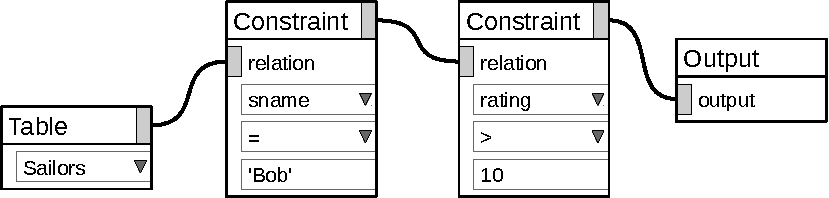
\includegraphics[width=0.9\textwidth]{resources/Conjunction.pdf}
  \caption{Conjunction by linking multiple constraints}
  \label{fig:conjunction}
\end{figure}

DFQL deals with this issue by using text-based constraints. This allows for arbitrarily complex predicates, but as discussed earlier, significantly complicates correctness validations.

\subsubsection*{Joins}
In Section~\ref{sec:nodes}, we designed the join node in such a way that it can handle all different types of joins. This is achieved by using a dynamic interface that adjusts the parameters depending on the type of join. Interestingly, the interface for the $\theta$-join turns out to be almost exactly the same as the interface for the constraint node. This makes sense, if we think of the $\theta$-join as simply a condition across multiple tables, which therefore requires a join. Accordingly, we can argue that instead of providing two mostly identical nodes, we should combine the functionality into one. Combining nodes is generally a good thing, as keeping the number of nodes low should, in theory, lead to a more user-friendly tool. On the other hand, the complexity of each individual node should be kept as low as possible and the behavior should be consistent and sensible. For instance, using a union operator to model a boolean disjunction is semantically correct, but not intuitively clear. In this case however, again using the intuition that a $\theta$-join is simply a condition across tables, combining the two nodes does not obscure their functionality. However, the question remains whether the combination can be performed without significantly increasing the complexity.

\begin{figure}[h]
  \centering
  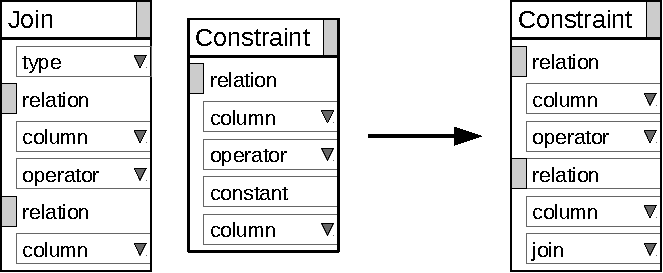
\includegraphics[width=0.7\textwidth]{resources/ConstraintNew.pdf}
  \caption{Combining join and constraint}
  \label{fig:constraint_new}
\end{figure}

Figure~\ref{fig:constraint_new} shows how the two nodes could be combined. The new constraint node contains the same number of parameters as the join node and one more than the basic constraint node. Furthermore, in order to constrain two columns of the same relation, we now need to attach the relation to both relation inputs. On the other hand, defining a join implicitly, based on a condition is potentially far more intuitive to users unfamiliar with the relational algebra and therefore should have a positive impact on usability. While EasyQuery also features an implicit join, there are a number of notable differences. Both query builders implicitly create a join for constraints across multiple tables. However, EasyQuery joins the tables based on foreign key relations and additional information provided with the schema, while the approach taken here simply joins the tables that are involved in the condition. This approach is a lot more flexible and grants the user more control over the construction of the query. For instance, it is powerful enough to express a self-join, something that cannot be modeled in EasyQuery. Additionally, the approach is also a lot more transparent, which is especially useful for more experienced users.

Up to now, the new node only properly covers the $\theta$-join leaving out natural, semi- and anti-joins. All three remaining types join the tables based on column names and therefore don't require any additional inputs. This behavior cannot be properly expressed using the current layout of the new constraint node. Therefore, we could either choose to keep a simplified version of the previous join node or alternatively drop support for these types of joins altogether. Another approach is to introduce a new type of join that combines characteristics of both the $\theta$- and semi-join. It accepts two relations and a condition and returns a relation that contains all the rows from the first relation for which there exists at least one row in the second table for which the specified condition is satisfied. In essence, this can be understood as a semi-join that uses a freely specified join condition instead of an equijoin based on column names. In fact, this behavior might be preferable due to the fact that it gives the user more control over the join condition used. The anti-join can be implemented analogously. The only join type left is the natural join. However, semantically speaking, a natural join is simply a special case of an equijoin which is itself a special case of a $\theta$-join which is already covered by the node. Additionally, the argument that joining based on column names leaves the user with little control applies to the natural join as well. In conclusion, keeping the join node for the sole purpose of supporting the natural join is not justified and we instead drop the feature.

\subsubsection*{Aggregation and Projection}
In addition to the changes applied so far, we also combine the aggregation and projection nodes. Unlike the combination of the constraint and join nodes, which was based on usability concerns and therefore non-essential, combining aggregation and projection is required in order to provide the full functionality. The assembly line metaphor used so far suggests that all operations that are applied to a relation take effect immediately. For instance, when a constraint is applied to a relation, the rows that do not satisfy the constraint are removed immediately. Likewise, an aggregation is applied directly, effectively changing the number of tuples in the relation. However, these two examples are treated differently by the query generator. The constraint results in a query that can still be modified. For instance, two constraints applied one after the other will result in a single query, without any use of subqueries. Aggregation on the other hand ``finalizes'' a query, meaning that any subsequent nodes may not change it in any way. For instance, a constraint on an aggregated query will create create a new query, using the aggregated one as a subquery. This is due to the fact that while many of the relational operators are commutative, aggregation is not. For example, assume that we want to rename a column and apply a constraint to a relation. In that case, the execution order of the two operations will not change the outcome. However, if we instead aggregate the column and apply the constraint, the order does indeed matter. Therefore, the output produced by the aggregation node has to be treated as a subquery. We use the simple query in Listing~\ref{lst:sname} to illustrate the problem and why it can be solved by combining the aggregation and projection nodes.

\begin{codeex}[caption=Example query,label=lst:sname]
SELECT sname
FROM Sailors;
\end{codeex}

Aggregating the query by applying COUNT to $sname$ can result in the two different queries shown in Listing~\ref{lst:agg_sname}.

\begin{codeex}[caption=Possible results of applying COUNT to \textit{sname}, label=lst:agg_sname]
SELECT COUNT(sname)
FROM Sailors;

SELECT sname, COUNT(sname)
FROM Sailors
GROUP BY sname;
\end{codeex}

Both queries return completely different results. The first query returns the number of sailors stored in the table while the second one returns the number of occurrences of every name in the table. However, both queries are perfectly reasonable, yet there is no way for the user to influence which of the two is going to be generated, which would result in a considerable loss of power. Combining aggregation and projection solves this issue, because it allows the user to exactly specify the desired query. In the example, since projection and aggregation happen simultaneously, the user can decide manually whether or not to include $sname$ in the projection. The layout of the new node is relatively straightforward and depicted in Figure~\ref{fig:select_new}.

\begin{figure}[h]
  \centering
  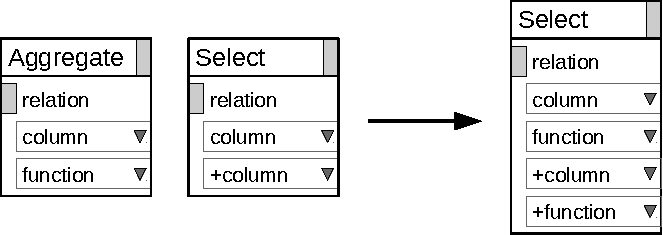
\includegraphics[width=0.7\textwidth]{resources/SelectNew.pdf}
  \caption{Combining aggregation and projection}
  \label{fig:select_new}
\end{figure}

DFQL handles this issue by adding an additional input to the aggregation node that takes a list of columns to be grouped which is quite similar to the approach taken here. However, since that node cannot be used to project columns without aggregating, DFQL retains an additional pure projection node.

\subsubsection*{Aliasing}
\label{sec:aliasing}
Due to the fact that SQL uses column names as unique identifiers, aliasing can result in unexpected behavior. Consider the example query in Listing~\ref{lst:drop_col}.

\begin{codeex}[caption=Query that drops column on join, label=lst:drop_col]
SELECT *
FROM Sailors s INNER JOIN Reserves r ON s.sid = r.sid;
\end{codeex}

Despite the fact that both tables contain a column named $sid$, the output relation only contains one such column. In this example, this is perfectly reasonable, due to the fact that the two columns are equi-joined and therefore identical. That is not necessarily the case though. Self-joins in particular will often cause columns to be dropped and thus require extensive renaming. Interestingly, the fact that any data is lost is irrelevant to the query builder, as it is oblivious to the data anyway. However, in order to keep track of typing information, it needs to know which of the two columns is dropped. This is relevant for set operations, where the types of all columns need to match.
One way to completely avoid this problem is by making sure that no column will get dropped in the first place. A simple technique to achieve this, is to generate generic aliases for every column. While this approach is very effective, it results in bloated queries, due to the fact that every column will be projected separately. This significantly reduces query readability and should therefore be avoided. Instead, aliases should only be generated when necessary, which requires extra logic to keep track of column names during joins.

\subsection{Correctness}
\label{sec:correctness}
One focus of this thesis is to design QENoBI in such way that it produces syntactically correct SQL queries. This has a number of influences on the design process. First off, we need to avoid text based inputs whenever possible. In practice, apart from constants, all inputs are based in drop-down lists and therefore a bounded number of inputs, eliminating the need for text analysis.

Using the assembly line metaphor, ensuring correctness is relatively simple, as every change in the program is immediately executed. Therefore, if an error should occur, it would be recognized immediately after the change is applied to the program. In practice however, query builders often operate only on the schema of the database and output an SQL query that is subsequently run on a DBMS. Therefore, the query builder has to consider all the issues that could potentially arise during the execution, assuming the worst possible scenario. For instance, the situation discussed in Section~\ref{sec:issues} about aliasing, where columns are dropped unintentionally due to identical naming, is relatively rare and therefore won't be an issue for most queries. Nonetheless, the query builder has to run meticulous checks in order to make sure that no issues will arise.

Query correctness can be divided into two parts, syntactical and semantical correctness. Achieving syntactical correctness is mostly dependent on the choice of query generator, which will be discussed in the section about query generation. Semantical correctness on the other hand is mostly handled by the nodes themselves. Due to the fact that most query builders, including the one presented here, are limited to the information available in the schema, semantical checks are mostly limited to typing. For example, the query builder could make sure that if the first column in a comparison is an integer, the second column has to be an integer as well. However, SQL typing is very weak and consequently, the presented example is actually perfectly valid in SQL. This raises the question, whether typing should be modeled to coincide with typing in SQL, or a more strict approach should be taken. For reference, EasyQuery uses a much stronger typing system than SQL. For instance, text comparison is limited to the equality, NULL and LIKE operators. This seems reasonable, but might alienate database users who are used to being able to use the types of comparisons used in the example. This is amplified by the fact that database schemas are often very old and inconsistent. For instance, an application might use text columns to store phone numbers in one table and integers in another. In this case, strong typing would make it impossible to define constraints across the two tables. Therefore, we choose to adhere to the weaker SQL typing model.

An interesting question is how to enforce correct typing in the interface. If possible, we want to implement typing in the interface in such a way that it is impossible to construct a semantically incorrect query. The first step to achieve this goal is to ensure that an input can only be attached to a node if the resulting query is semantically sound. Due to the fact that we have chosen a very weak typing system, this is relatively simple. For instance, all relations attached to a merge node must have the same number of columns. Had we chosen to adapt more strict typing rules, we would have to ensure that the types are identical as well. To implement this behavior, we introduce the idea of a domain as the set of possible values of a parameter. For a connection to be valid, the value of the source of the connection must therefore occur in the domain of the parameter.

\begin{figure}[h]
  \centering
  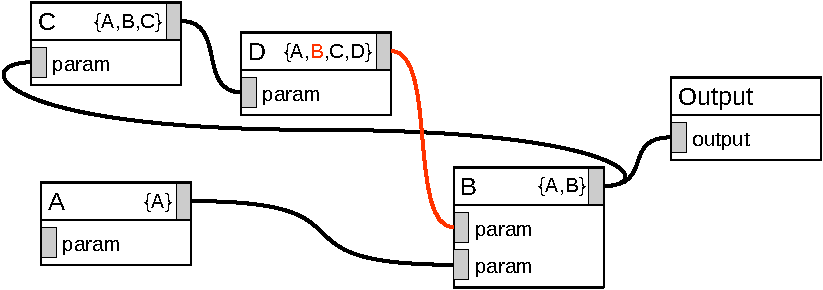
\includegraphics[width=0.8\textwidth]{resources/Cycle.pdf}
  \caption{Cycle detection using dependency sets}
  \label{fig:cycle}
\end{figure}

This method can also be applied to solve another issue that has not been addressed yet. Dataflow programming allows the creation of cycles in the program graph to model iterative computations. However, since queries on the relational algebra are always tree-shaped, we need to ensure that no cycles can be created. A straightforward way to implement this, is to maintain a set of dependencies in every node. Looking at the tree structure, the dependency set of node $N$ contains all nodes in the subtree with root $N$, including $N$ itself. In other words, the dependency set of node $N$ is the union of the sets of all its children. This procedure can be applied directly, as the query is generated bottom-up. A new connection is now valid, if the target node does not appear in the dependency set of the source node. In Figure~\ref{fig:cycle} connecting $D$ to $B$ is invalid, because $B$ is in the dependency set of $D$.

These two measures combined ensure that all connections that can be drawn are also valid. However, the user might still change parameters in the nodes leading to incorrect program states. One way to circumvent this issue, is by applying typing constraints not just to inputs and outputs but any parameter in general. The options displayed in the drop-down lists could then be limited to show non-conflicting options only. For instance, the relation selection in a Table node that is connected to a Merge node could then be limited to relations containing the correct number of columns. This process is somewhat more elaborate than the ones discussed in the previous paragraphs, as it requires type inference across multiple nodes. A similar approach, used to limit options in subnodes, is explained in more detail in Section~\ref{sec:subnodes}.

\subsection{Subnodes}
\label{sec:subnodes}
One of the major benefits of dataflow programming is the concept of subnodes, allowing the grouping of nodes into a new node that combines their functionality. To understand how subnodes can greatly improve the usability, abstraction and maintainability of the query builder, we will create a subnode that solves a problem that is often used to describe why SQL is a difficult language to learn. Aggregation functions are used to retrieve the maximum or minimum value of a column. For instance, \texttt{MAX} can be used to obtain the age of the oldest sailor. However, the desired information is often not just the value of the column itself but the entire row. In the example query, we only get the age, but the name of the oldest sailor. To obtain the entire tuple, the somewhat obscure query shown in Listing~\ref{lst:maxQ} is required. Figure~\ref{fig:maxQ} shows the same query implemented using QENoBI.
\begin{codeex}[caption=Retrieve oldest sailor in SQL, label=lst:maxQ]
SELECT *
FROM Sailors
WHERE age = (SELECT MAX(age) FROM Sailors);
\end{codeex}

\begin{figure}[h]
  \centering
  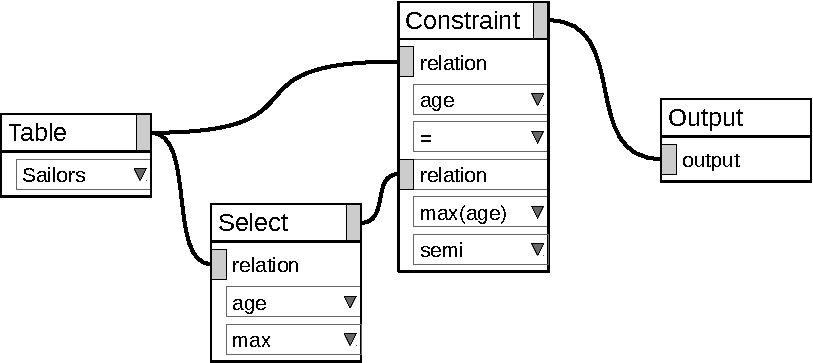
\includegraphics[width=0.8\textwidth]{resources/MaxQ.pdf}
  \caption{Retrieve oldest sailor without use of subnodes}
  \label{fig:maxQ}
\end{figure}

While it is clear that this query produces the desired result, it is rather cumbersome. Note that this query employs the hybrid join introduced in Section~\ref{sec:issues}. Therefore, we introduce a new Maximize node which returns all the rows where a certain column reaches the highest value. The query implemented using this new node is presented in Figure~\ref{fig:maxQ_sub}.

\begin{figure}[h]
  \centering
  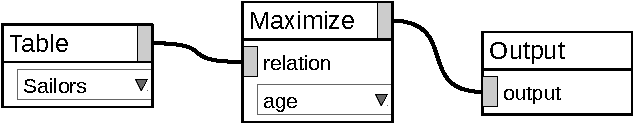
\includegraphics[width=0.6\textwidth]{resources/MaxQSub.pdf}
  \caption{Retrieve oldest sailor using Maximize subnode}
  \label{fig:maxQ_sub}
\end{figure}

In order to able to create a subnodes that implements this functionality, we need a way to indicate that a certain value is not available yet and will be provided by the end-user. We refer to these as \emph{deferred values}. Since all the deferred values need to be initialized in order to be able to construct the query, the mask of the subnode, i.e. the user interface of the node that represents the group of nodes, is simply a list of all deferred values. For instance, if a subnode contains two deferred parameters, a relation and a column, then the mask of the subnode is a node that contains the same two parameters. To access the values from within the subnode, we introduce a new primitive node, the input node. It contains the same parameters as its subnode but as outputs instead of inputs. As such, it is the only node that contains multiple outputs. Similar to the output node, there can only be one input node in every query. The Maximize subnode using the new input node and two deferred parameters \emph{r1} and \emph{c1} is depicted in Figure~\ref{fig:subnode}.

\begin{figure}[h]
  \centering
  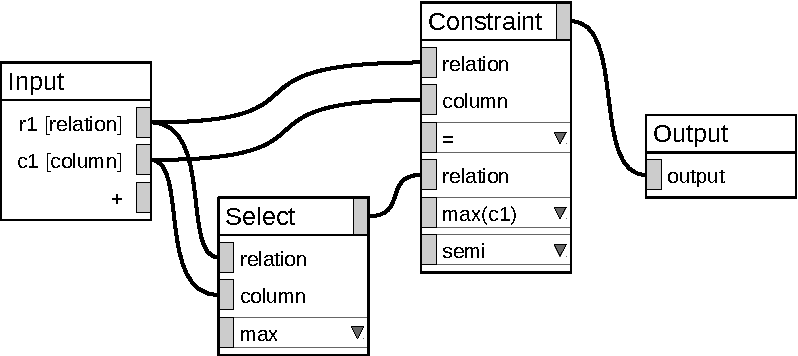
\includegraphics[width=0.8\textwidth]{resources/Subnode.pdf}
  \caption{Internals of the Maximize subnode}
  \label{fig:subnode}
\end{figure}

One of the first things to note, is that relations are no longer the only parameters to feature an attachment point. This is due to the fact that any type of value, including columns and operators, can be deferred. This might seem to conflict with the operational closure property discussed earlier in Section~\ref{sec:pow_df}. However, non-relation parameters can only be outputs in the input node and cannot be connected to the output node. Therefore, every node except for the input node will output a relation. Furthermore, the input node is simply a visualization of the data passed to the subnode and during query generation, all deferred values are initialized, effectively removing all non-relation connections.

The example in Figure~\ref{fig:subnode} displays a number of different features related to subnodes and parameter deferring. First off, the Input node displays the same parameters as the subnode, as established in the previous paragraph. Unique identifiers are automatically assigned. Note that these are not column aliases but are instead used to distinguish multiple columns. In other words, the identifier is the column or relation name to be used inside the subnode, as the real names are not known during construction of the subnode and change depending on the query the subnode is used in. If a parameter is deferred, i.e. an a connection is drawn from a parameter of the input node to its input, all input elements such as drop-down lists or text fields are removed to indicate that the parameter can no longer be set manually. One parameter that needs to be addressed separately is the penultimate parameter in the constraint node, which defines the second column to be used in the equality predicate. The parameter is interesting, because it is set to the aggregation of a deferred column. To understand how this works, we need to examine the output relation of the Select node. While both the relation and column input of the Select node are deferred, the output is clearly defined. This is due to the fact that the Select node always produces a relation containing a single column $max(c1)$ regardless of whether column $c1$ is deferred. As a consequence, the output can be used as before. Another interesting case is depicted in Figure~\ref{fig:part_def}.

\begin{figure}[h]
  \centering
  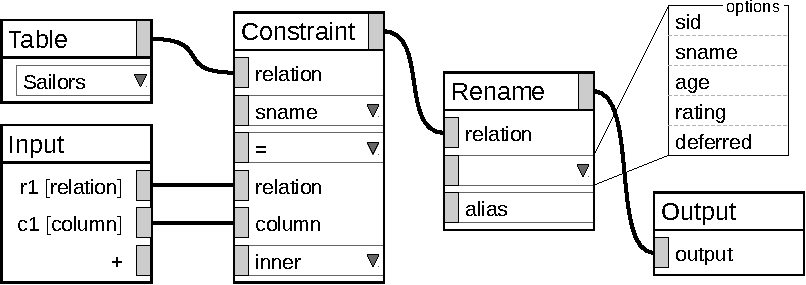
\includegraphics[width=0.8\textwidth]{resources/PartDef.pdf}
  \caption{Partially deferred relation containing placeholder column}
  \label{fig:part_def}
\end{figure}

In this example, a deferred relation is joined to a non-deferred one using a constraint node, resulting in a partially deferred relation. While some of the columns in the output relation, specifically those from the sailors table, are known, others are not. Therefore, the drop-down list in the Rename node needs to take into account that the user might want to rename a deferred column. This is achieved by adding a new option \textit{deferred} to the list. Selecting this option then creates a new parameter in the input node and automatically connects it to the parameter in the Rename node.

\begin{figure}[h]
  \centering
  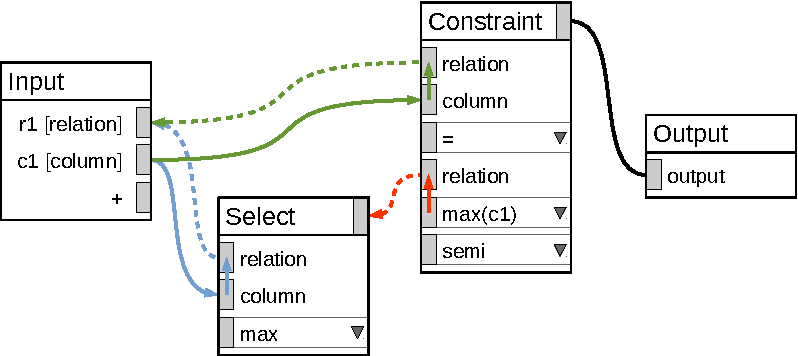
\includegraphics[width=0.8\textwidth]{resources/Dependencies.pdf}
  \caption{Visualisation of parameters dependencies}
  \label{fig:dependencies}
\end{figure}

One question that hasn't been addressed at all, is how the options in the column drop-down lists are calculated. For primitive nodes, the process is relatively straightforward. Every column parameter is assigned a source relation which defines the set of columns that can be selected. For instance, the column parameter of the Rename node is limited to the columns that occur in the relation that is attached to the node's relation parameter. Nodes that contain an arbitrary number of column parameters, such as the Sort and Select nodes, have only one relation parameter that is used as the source relation for all columns parameters. Therefore, all dependencies are internal and can be handled by every node individually. However, taking into account the changes made to support subnodes, this is no longer the case. In the Maximize subnode for instance, the second parameter is used in two different nodes and therefore has to satisfy the criteria of both. To better understand the problem, Figure~\ref{fig:dependencies} visualizes the dependencies in the Maximize subnode. The solid arrows represent column dependencies, indicating the source relation of a column parameter. Once the source relation has been identified, the dotted arrows then indicate the origin of this relation. Since both the green and the blue dependency need to be considered, the only columns that are valid are the ones that occur in both source relations. Otherwise, if a column was to be chosen that is not present in one of the source relations, we would end up with a semantically incorrect query. Therefore, given the set $D_c$ of all dependency relations $r$ of a column parameter $c$, the set of valid options is defined as $$options(c) = \bigcap_{r \in D_c} cols(r)$$
In the example, both dependencies result in the same origin relation and as a result, the set of valid options is given by $options(c1) = cols(r1) \cap cols(r1) = cols(r1)$.

In order to generate a query, all deferred parameters should be initialized as the behavior is undefined otherwise. However, queries that contain deferred and non-initialized parameters could be translated into stored procedures, if that feature is available on the SQL platform used. Using this approach, the interface can be unified, eliminating the differences between creating a subnode or a query.

Overall, the examples show that subnodes have a profound, positive impact on the versatility of the query builder. The ability to group the functionality of multiple nodes into one not only allows the simplification of frequently used tasks but also serves to significantly increase the level of abstraction as demonstrated by the Maximize example.

\subsection{Query Generation}
So far, we have addressed the architecture and the functionality of the query builder, but not the generation of the query itself. There are many different approaches that can be used to generate SQL queries from tree based declarations and choosing the right one is crucial. The approach taken here relies on a formal grammar to model the query.\\
Due to the fact that the interface limits the types of constructs that can be expressed by the query builder, the language of the resulting SQL queries can be expressed in a relatively compact, context-free grammar. The rules of the grammar are listed in Table~\ref{tab:grammar}. Note that some of the trivial rules, such as \textit{Arit} which covers arithmetic expressions, are omitted to keep the number of rules manageable.
\begin{table}[h]
\centering
\begin{tabu} to \textwidth {l c l}
\toprule
\textit{Set}				& $\rightarrow$	& '(' \textit{Set} \textit{SetOp} \textit{Set} ')' \textbar~\textit{Query} \\[2pt]
\textit{Query}				& $\rightarrow$ & \textit{Select} '\texttt{DISTINCT}'? \textit{From} \textit{Where}? \textit{Group}? \textit{Order}? \textit{Limit}? \\[2pt]
\textit{Select}				& $\rightarrow$	& '\texttt{SELECT}' ( \textit{Expression} ( '\texttt{AS}' \textit{Ident} ) )* \\[2pt]
\textit{From}				& $\rightarrow$	& '\texttt{FROM}' \textit{Relation} \\[2pt]
\textit{Where}				& $\rightarrow$	& '\texttt{WHERE}' \textit{Condition} \\[2pt]
\textit{Group}				& $\rightarrow$	& '\texttt{GROUP BY}' \textit{Column}* \\[2pt]
\textit{Order}				& $\rightarrow$	& '\texttt{ORDER BY}' ( \textit{Column SortType}? )* \\[2pt]
\textit{Limit}				& $\rightarrow$	& '\texttt{LIMIT}' \textit{Number} ( '\texttt{OFFSET}' \textit{Number} )? \\[2pt]
\textit{Relation}			& $\rightarrow$	& \textit{Table} \textbar~\textit{Join} \\[2pt]
\textit{Table}				& $\rightarrow$	& ( \textit{Ident} \textbar~'(' Set ')' ) \textit{Ident} \\[2pt]
\textit{Join}				& $\rightarrow$	& '(' \textit{Relation} \textit{JoinType} \textit{Relation} '\texttt{ON}' \textit{Condition} ')' \\[2pt]
\textit{Condition}			& $\rightarrow$	& \textit{Connective} \textbar~\textit{Comparison} \textbar~\textit{Exists} \\[2pt]
\textit{Connective}			& $\rightarrow$	& \textit{Condition} ( '\texttt{AND}' \textbar~'\texttt{OR}' ) \textit{Condition} \\[2pt]
\textit{Comparison}			& $\rightarrow$	& \textit{Expression} \textit{CompOp} \textit{Expression} \\[2pt]
\textit{Exists}				& $\rightarrow$	& '\texttt{NOT}'? '\texttt{EXISTS}' '(' \textit{Set} ')' \\[2pt]
\textit{Expression}			& $\rightarrow$	& \textit{Column} \textbar~\textit{Constant} \textbar~\textit{Aggregate} \textbar~\textit{Arit} \textbar~\textit{Function} \\[2pt]
\textit{Column}				& $\rightarrow$	& \textit{Ident} '.' \textit{Ident} \\[2pt]
\textit{Aggregate}			& $\rightarrow$	& \textit{AggType} '(' \textit{Expression} ')' \\[2pt]
\midrule
\textit{SetOp}				& $\rightarrow$ & '\texttt{UNION}' \textbar~'\texttt{INTERSECT}' \textbar~'\texttt{MINUS}' \\[2pt]
\textit{SortType}			& $\rightarrow$ & '\texttt{ASC}' \textbar~'\texttt{DESC}' \\[2pt]
\textit{JoinType}			& $\rightarrow$ & ( '\texttt{INNER}' \textbar~( '\texttt{LEFT}' \textbar~'\texttt{RIGHT}' \textbar~'\texttt{FULL}' ) '\texttt{OUTER}' ) '\texttt{JOIN}'\\[2pt]
\textit{CompOp}				& $\rightarrow$ & '\texttt{=}' \textbar~'\texttt{<>}' \textbar~'\texttt{<}' \textbar~'\texttt{<=}' \textbar~'\texttt{>}' \textbar~'\texttt{>=}' \\[2pt]
\textit{AggType}			& $\rightarrow$ & '\texttt{MIN}' \textbar~'\texttt{MAX}' \textbar~'\texttt{AVG}' \textbar~'\texttt{SUM}' \textbar~'\texttt{COUNT}' \\[2pt]
\bottomrule
\end{tabu}
\caption{Grammar covering the limited SQL language}
\label{tab:grammar}
\end{table}
The language produced by this grammar over-approximates the language of all syntactically correct queries that can be constructed using the query builder. For instance, using the production rules, we can derive the incorrect query shown in Listing~\ref{lst:grammar_incorrect}.

\begin{codeex}[caption=Incorrect query derivable using the rules in Table~\ref{tab:grammar}, label=lst:grammar_incorrect]
SELECT MIN(MAX(age))
FROM Sailors;
\end{codeex}

This fact needs to be considered when implementing the query generation part of each node. This particular query for instance can never occur due to the fact that the Select node ``finalizes'' the query, meaning that its output may only be treated as a subquery by subsequent nodes. Therefore, if two aggregations are performed in succession, we obtain the correct query shown in Listing~\ref{lst:grammar_correct}.

\begin{codeex}[caption=Correct syntax for the query in Listing~\ref{lst:grammar_incorrect}, label=lst:grammar_correct]
SELECT MIN(a1)
FROM (SELECT MAX(age) AS a1 FROM Sailors);
\end{codeex}

Following the assembly line metaphor, any output produced by a node is a relation. This also implies that any output produced by a node can be connected to the Output node, providing a complete query. Therefore, the query is not built progressively but instead, the Table node creates the base query shown in Listing \ref{lst:base_query} which is then modified by subsequent nodes. The Sort node for instance simply attaches the \texttt{ORDER BY} clause to its input query.

\begin{codeex}[caption=Base query generated by the Table node, label=lst:base_query]
SELECT *
FROM table_name;
\end{codeex}

The resulting structure can be understood as an abstract syntax tree, a structure that is commonly used in compiler design. Consequently, query generation can then be implemented using a visitor or simply by traversing the tree.

It is important to note that subnodes do not need to be handled separately when generating the query. This is due to the fact that subnodes are merely a visual abstraction and only exist in the GUI but not in the logic. Therefore, ``virtual'' nodes that are located inside a subnode are handled exactly the same way as ``physical'' nodes and thus no changes to the logic of query generation are required.

%---------------
%Implementation
%---------------

\chapter{Implementation}
\label{ch:impl}

\section{Specification}
This chapter discusses a proof of concept implementation of QENoBI. It is based on a limited feature set that reduces the scope but nonetheless allows to verify the practical viability of the major concepts developed in Chapter~\ref{ch:approach}.

\subsection{Features}
The key purpose of the implementation is to verify the practicality of the concept. Therefore, rather than implementing every feature that is part of the specification, we focus on a limited number of features that collectively cover as many aspects as possible. The Limit and Sort nodes for instance are very similar in functionality and therefore it suffices to implement one of the two to validate the principle. Limiting the scope in this way leads to a greatly simplified but inevitably fragmentary implementation. Most prominently, subnodes are not implemented, which considerably limits our ability to assess the implications of the concept. However, as mentioned in Section~\ref{sec:subnodes}, subnodes have no impact on the expressive power of the query builder and are by far the most complex feature implement. As a consequence, subnodes were ultimately removed from the feature set. However, this does not mean that it is impossible to implement subnodes as specified. Instead it is a result of the fact that the architecture chosen for the implementation is neither flexible nor powerful enough to support a proper implementation of subnodes. Additionally, expressions are also missing from the implementation, as they too require a more flexible structure than the rest of the primitive nodes. Aside from these dropped features, most of the functionality of the specification is present in the implementation and is discussed more thoroughly in Chapter~\ref{ch:eval}

\subsection{Technology}
Web-based applications have made great strides in the past decade and increasingly used to implement functionality that used to be exclusive to stand-alone applications. This is due to the fact that web-based applications combine a number of very beneficial characteristics such as platform independence, ease of use and distribution as well as maintenance. The rise in popularity has been enabled by the constantly increasing performance and the ubiquity of web browsers and internet access in general. Since web applications are websites after all, they are also very well suited for GUI-intensive applications. Therefore, QENoBI is implemented as a web-based application. One consequence of this design decision, is that the query builder is limited to the creation queries and cannot be used to display the results directly. However, this functionality could be added as future work, by combining the query builder with a web-accessible DBMS backend.

Due to vendor-specific differences in SQL, it is impossible to generate SQL code that is guaranteed to run on all DBMS. Therefore, QENoBI specifically produces code that is optimized to run on PostgreSQL, which is known for its power and standards-compliance. It is also free and open source software, released under the terms of the PostgreSQL License.

\section{User Interface}
The commercial query builders discussed in \ref{sec:requirements}, EasyQuery and ExtJS, both feature relatively ``crowded'' user interfaces as shown in Figures~\ref{fig:easyquery}~and~\ref{fig:extjs}. This is problematic, as it might take users a while to get used to the interface, or even worse, discourage them from using the tool altogether. In order to avoid these issues, QENoBI features a very lightweight interface shown in Figure~\ref{fig:qenobi}.

\begin{figure}[h]
  \centering
  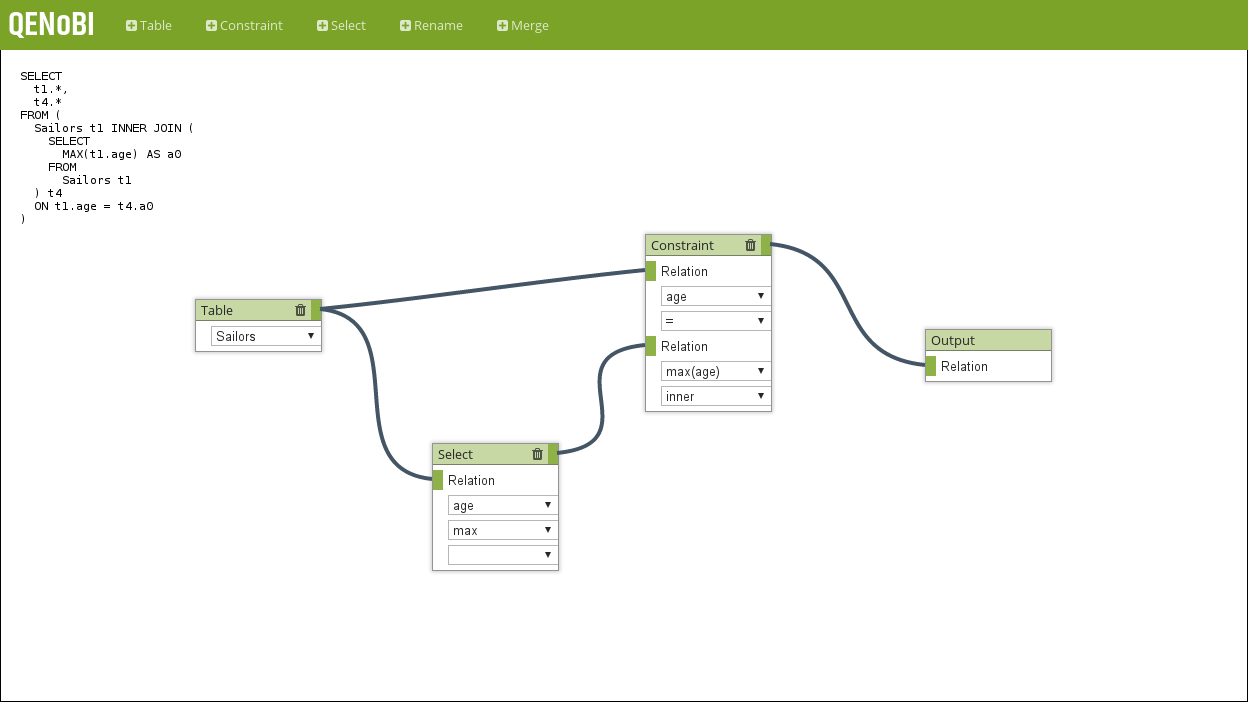
\includegraphics[width=\textwidth]{resources/QENoBI.png}
  \caption{A screenshot of the Maximize query implemented in QENoBI}
  \label{fig:qenobi}
\end{figure}

The overall application design mimics the look of modern web pages, using a navbar as the primary, and in this case only structural element. The output query is displayed directly on the main container, a behavior that is inspired by a similar feature found in Blender. Due to this very minimalistic interface, the majority of the screen is left to the query editing container. The node layout is very similar to the design used in Chapter~\ref{ch:approach}.

\section{Architecture}
In this section, we discuss the general architecture of the application. This includes the outline of the program structure, the libraries and some of the functionalities.

\subsection{Program Structure}
The application is written entirely in JavaScript and makes heavy use of its prototyping system. As such, most theoretical concepts in the specification have a distinct counterpart in the implementation. The GUI is strictly separated from the logic part of the application. While this is good practice in general, it is a requirement for QENoBI if subnodes are implemented. This is due to the fact that nodes contained in subnodes should be treated identically to nodes that are visible in the GUI, thus requiring a clear separation of the node logic. The basic node structure is depicted in Figure~\ref{fig:node_structure}. The dotted arrows represent pointers between the components.

\begin{figure}[h]
  \centering
  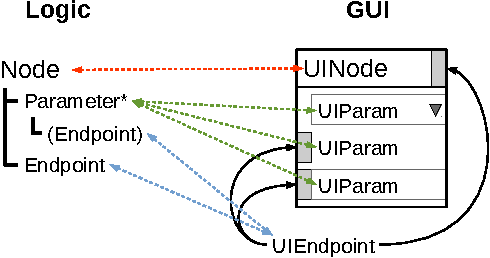
\includegraphics[width=0.6\textwidth]{resources/NodeStructure.pdf}
  \caption{Structure of the node}
  \label{fig:node_structure}
\end{figure}

Since subnodes are not part of the feature set of the implementation, this separation is not a necessity but still beneficial as it leads to cleaner code in the logic part.

\subsection{Communication}
Communication in dataflow programming is usually handled by message passing. This is consistent with the assembly line metaphor, where workers process their inputs once they are available and send the result to the next node on the assembly line. This is very beneficial in concurrent settings dealing with continuous data streams, as message passing does not rely on procedure calls but is usually implemented using channels.

Since query builder are essentially compilers, data streams and parallelism are of less concern. Therefore, QENoBI uses the observer pattern, which is employed for communication between nodes as well as node internal updating. Every component maintains a list of observers which are notified if the value of the component changes. Since neither subnodes nor strong typing are implemented, messages are always passed bottom-up until they reach the ``drain'' of the query graph, the Output node. In a setting where two-way communication is required, the observer pattern does not suffice, as it cannot handle circular dependencies.

\subsection{Libraries}
QENoBI relies on jsPlumb\footnote{https://www.jsplumbtoolkit.com}, a collection of libraries that provides means to build graph-based interfaces. This includes its own dragging library which natively supports touch events. It is dual-licensed under the MIT and GPLv2 licenses and hosted on GitHub\footnote{https://www.github.com/sporritt/jsplumb/}.

\subsection{Query Generation}
The query generation code is directly based on the grammar rules listed in Table~\ref{tab:grammar}. A few simplifications aside, every rule in the grammar corresponds to a class in the implementation. The simplified syntax tree generated for the query in Listing~\ref{lst:syntax_tree} is depicted in Figure~\ref{fig:syntax_tree}.

\begin{codeex}[caption=Example query that produces the syntax tree in Figure \ref{fig:syntax_tree}, label=lst:syntax_tree]
SELECT *
FROM (
    (Sailors s INNER JOIN Reserves r ON s.sid = r.sid) j
    INNER JOIN Boats b
    ON j.bid = b.bid
  )
\end{codeex}

\begin{figure}[h]
  \centering
  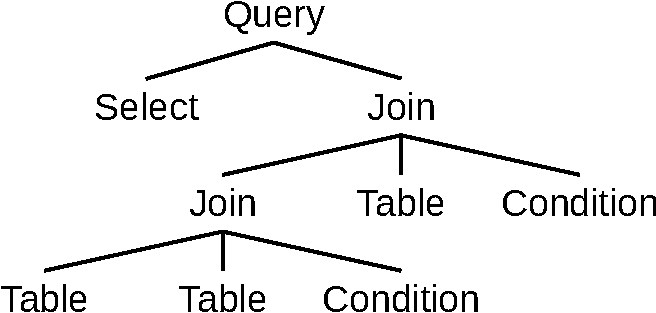
\includegraphics[width=0.6\textwidth]{resources/SyntaxTree.pdf}
  \caption{Simplified syntax tree of the query in Listing \ref{lst:syntax_tree}}
  \label{fig:syntax_tree}
\end{figure}

This syntax tree can now be traversed using DFS to generate the query. For this purpose, every class contains a \texttt{getQuery()} function that constructs and returns a partial query by calling \texttt{getQuery()} on its children. Therefore, calling \texttt{getQuery()} on the root of the tree returns the complete query.

%---------------
%Evaluation
%---------------

\chapter{Evaluation}
\label{ch:eval}

\section{Evaluation Set}
\label{sec:eval_set}
In this chapter, we evaluate the performance of QENoBI. The test set used in Section~\ref{sec:test_set} can be understood as a training set for QENoBI since the list of features is derived from it. As a consequence, testing whether QENoBI performs well on these queries is not very informative, as it was designed with these queries in mind. Therefore, we need to extend the test set with ``fresh'' queries that have not been tested before. The  queries that make up this evaluation set are chosen by similar criteria. As before, we are interested in covering as many features as possible while remaining unbiased. However, since basic functionality is already covered in the original set, the additional queries are more complex on average. Table~\ref{tab:eval_set} lists an overview of the extended set and the actual queries can be found in the appendix.

\begin{table}[h!]
\centering
\begin{tabu} to \textwidth {l c c}
\toprule
\textbf{Source}								& \textbf{Complexity}	& \textbf{Quantity}	\\
\midrule
Database Management Systems					& low					& 9					\\
Wikipedia									& varies				& 2					\\
Typo3										& medium				& 3					\\
Joomla										& medium				& 1					\\
LedgerSMB									& varies				& 4					\\
Microsoft Benchmark							& high					& 2					\\
\midrule
Drupal										& low					& 1					\\
WordPress									& medium				& 3					\\
MusicBrainz									& varies				& 3					\\
LedgerSMB									& high					& 3					\\
TPC Benchmark								& high					& 3					\\
\bottomrule
\end{tabu}
\caption{Test Set (extended)}
\label{tab:eval_set}
\end{table}

\section{Results}
Using the evaluation set we now analyze the functionality of QENoBI. The results are listed in Table~\ref{tab:test_eval} along with the results of the other query builders that were evaluated on test set before. For every query that can be fully expressed, a query builder is awarded one point. Half points are awarded if a feature is not supported but could be added with minimal effort. This is equivalent to the 'possible' verdict in Table~\ref{tab:features}. For some queries, it is impossible to assess whether they can be implemented or not without additional information. For instance, since EasyQuery uses an implicit join, any join operations will work only if the particular join used is defined in EasyQuery's enhanced schema. These cases are interpreted as partial support and are counted as half a point. Note that the output query does not have to be equivalent to the target query in the test set. Instead, we test whether the query can be expressed semantically. Furthermore, QENoBI is listed twice where one column represents the implementation while the other one represents QENoBI according to the specification.

\begin{table}[h!]
\centering
\begin{tabu} to \textwidth {l c c c c c c}
\toprule
\textbf{Set}	& \textbf{\# of Q.}	& \textbf{EasyQuery}	& \textbf{ExtJS}	& \textbf{DFQL}	& \textbf{QENoBI-I}	& \textbf{QENoBI-S}	\\
\midrule
Test			& 20					& 11					& 12.5				& 17			& 14.5					& 19		\\
Evaluation		& 13					& 3.5					& 6					& 10			& 6.5					& 11		\\
\midrule
Total			& 33					& 14.5					& 18.5				& 27			& 21					& 30		\\
\bottomrule
\end{tabu}
\caption{Evaluation on the extended test set}
\label{tab:test_eval}
\end{table}

As expected, QENoBI performs extremely well on the original test set. 19 out of the 20 queries can be expressed using QENoBI based on the full specification. The remaining query contains a \texttt{DECODE} expression (Oracle's version of CASE) which is problematic, as it accepts an arbitrary amount of features, which cannot be expressed using the Expression node as specified. The proof-of-concept implementation achieves 14.5 points on the test set, emphasizing its limited functionality with respect to the specification. Nonetheless, it perform significantly better than both EasyQuery and ExtJS which attain 11 and 12.5 points respectively. It loses points for a number of different reasons, most prominently however due to the lack of expression support.

As mentioned in Section~\ref{sec:eval_set}, the queries in the evaluation set are more complex on average. This is mirrored in the test results, with all query builders covering a lower percentage of the queries. EasyQuery in particular only attains 3.5 out of 13 points which is mostly due to its rigid architecture, which for instance restricts the join operations possible. ExtJS and the implementation of QENoBI both cover roughly half of the queries. Interestingly though, the distribution of points differs quite significantly. ExtJS doesn't support complex constructs such as subqueries or set operations and consequently loses many points on structurally complex queries. QENoBI on the other hand, supports all these constructs but, as implemented, lacks expression support which results in a number of inexpressible queries. Taking the full specification into account, QENoBI performs significantly better. As with the test set, the only cases it cannot express are complicated expressions. In particular, the query in Listing~\ref{lst:project_constant} cannot be expressed in QENoBI. The issue is not located in the second column, as one might suspect, but the third. Specifically, the third column is projected ``out of thin air'' which cannot be expressed using the nodes as specified due to the fact that an expression node always replaces the columns it operates on.

\begin{codeex}[caption=Query projecting a constant, label=lst:project_constant]
SELECT
  name, 'V-' || vendornumber, 1
FROM
  lsmb12.vendor
GROUP BY
  name, vendornumber;
\end{codeex}

Based on the evaluation set we also evaluate QENoBI on the list of features in Table~\ref{tab:features}. The results are listed in Table~\ref{tab:features_eval} alongside the results obtained previously in Section~\ref{sec:feature_set} for comparison. Features that are part of the QENoBI specification but not present in the implementation are marked as `not implemented'.

\begin{table}[h!]
\centering
\begin{tabu} to \textwidth {l X[c] X[c] X[c] c | c X[c]}
\toprule
							& EasyQuery			& ExtJS				& DFQL				&&& QENoBI				\\
\midrule
\textbf{Relational Algebra}	&					&					&					&&&						\\
Projection					& \tc{g}{yes}		& \tc{o}{partial}	& \tc{g}{yes}		&&&	\tc{g}{yes}			\\
Selection					& \tc{g}{yes}		& \tc{g}{yes}		& \tc{g}{yes}		&&&	\tc{g}{yes}			\\
Rename						& \tc{g}{yes}		& \tc{g}{yes}		& \tc{g}{yes}		&&&	\tc{g}{yes}			\\
Natural Join				& \tc{o}{implicit}	& \tc{r}{no}		& \tc{o}{possible}	&&&	\tc{o}{possible}	\\
$\theta$-Join				& \tc{o}{implicit}	& \tc{o}{partial}	& \tc{g}{yes}		&&&	\tc{g}{yes}			\\
Outer Join					& \tc{o}{implicit}	& \tc{g}{yes}		& \tc{o}{possible}	&&&	\tc{g}{yes}			\\
Semi/Anti-Join				& \tc{r}{no}		& \tc{r}{no}		& \tc{o}{possible}	&&&	\tc{o}{not impl.}	\\
Aggregation					& \tc{g}{yes}		& \tc{g}{yes}		& \tc{g}{yes}		&&&	\tc{g}{yes}			\\
Subqueries					& \tc{o}{partial}	& \tc{r}{no}		& \tc{g}{yes}		&&&	\tc{g}{yes}			\\
Set Operations				& \tc{r}{no}		& \tc{r}{no}		& \tc{g}{yes}		&&&	\tc{g}{yes}			\\
\midrule
\textbf{SQL Features}		&					&					&					&&&						\\
Expressions					& \tc{r}{no}		& \tc{g}{yes}		& \tc{g}{yes}		&&&	\tc{o}{not impl.}	\\
Sort						& \tc{g}{yes}		& \tc{g}{yes}		& \tc{g}{yes}		&&& \tc{o}{not impl.}	\\
Limit						& \tc{r}{no}		& \tc{r}{no}		& \tc{o}{possible}	&&&	\tc{o}{not impl.}	\\
Distinct					& \tc{r}{no}		& \tc{r}{no}		& \tc{i}{}			&&&	\tc{g}{yes}			\\
\midrule
\textbf{Usability}			&					&					&					&&&						\\
Visual						& \tc{r}{low}		& \tc{o}{medium}	& \tc{g}{high}		&&&	\tc{g}{high}		\\
Abstraction					& \tc{o}{medium}	& \tc{r}{low}		& \tc{g}{high}		&&&	\tc{g}{high}		\\
Contextual					& \tc{g}{high}		& \tc{r}{low}		& \tc{r}{low}		&&&	\tc{g}{high}		\\
Correctness					& \tc{g}{high}		& \tc{r}{low}		& \tc{r}{low}		&&&	\tc{o}{not impl.}	\\
Readability					& \tc{o}{medium}	& \tc{g}{high}		& \tc{i}{}			&&&	\tc{g}{high}		\\
\bottomrule
\end{tabu}
\caption{Evaluation of QENoBI next to results from Section~\ref{sec:feature_set}}
\label{tab:features_eval}
\end{table}

Unsurprisingly, DFQL and QENoBI exhibit almost identical performance in the first two sections. This is due to the fact that they are both based on the dataflow paradigm. Both query builders manage to cover significantly more features of relational model than the other two query builders which are based on a more static approach. To be consistent with the evaluation process applied in Section~\ref{sec:feature_set}, the natural join is denoted as 'possible' even though we specifically decided to drop it in from the specification. This is due to the fact that the goal of the feature-based evaluation is to assess the power of the tool, i.e. how many of the features it can cover. Therefore, since adding support for the natural join is as simple as adding a new node, the feature is denoted as 'possible'. Although not present in the implementation, the specification of QENoBI also supports all the SQL specific features in the second category, with the exception of the cases discussed above. Finally, QENoBI significantly outperforms the other builders in the usability category. However, these results should be taken with a grain of salt due to the fact that usability is highly subjective and can only be properly assessed by a user study. Potential setups for such a study is discussed in Section~\ref{sec:user_eval}. While a complete usability assessment requires a thorough user study, certain parts of it can be examined independently. For instance, the architecture used in QENoBI enables correctness validation to be implemented, arguably resulting in a better user experience. Likewise, while the full potential of subnodes would have to be assessed by an independent set of test users, the example presented in Section~\ref{sec:subnodes} shows some very interesting results that could significantly impact the usability fot novice users.

\subsection{Strengths}

We take a closer look at two queries to show off some of the strengths of QENoBI. The first query, a modified query from the evaluation set, is shown in in Figure~\ref{fig:eval_query1} along with the implementation in QENoBI. The query is interesting because it requires a self-join, which is not supported by EasyQuery.

\begin{figure}[h]
\begin{codeex}[]
SELECT
  COUNT(*)
FROM
  Sailors t1, Sailors t2
WHERE
  t2.age > 20 AND t1.sid = t2.sid;
\end{codeex}

  \centering
  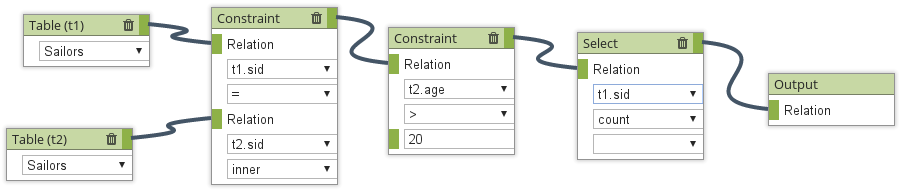
\includegraphics[width=\textwidth]{resources/EvalQuery1.png}
  \caption{Query featuring a self-join implemented in QENoBI}
  \label{fig:eval_query1}
\end{figure}

The second query shown in Figure~\ref{fig:eval_query2} is based on a query from the evaluation set as well. It demonstrates QENoBI's support for set operations.

\begin{figure}[h]
\begin{codeex}[]
SELECT *
FROM (
    SELECT sid, sname
    FROM Sailors
  UNION
    SELECT bid, bname
    FROM Boats
)
WHERE
  sname = 'Bob';
\end{codeex}

  \centering
  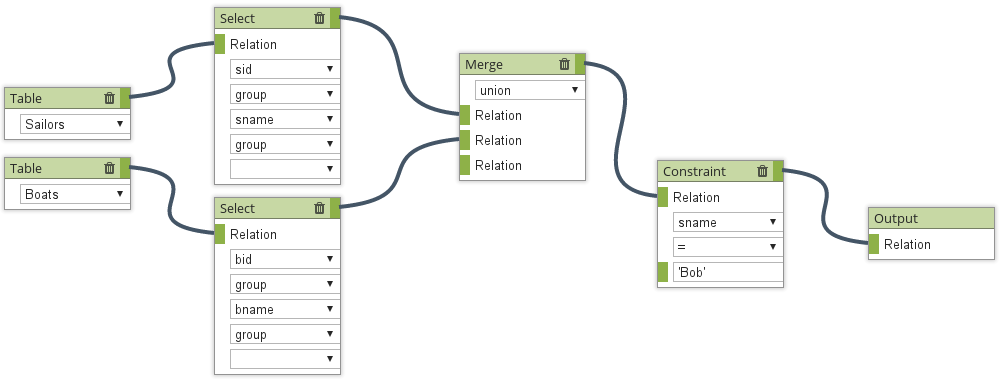
\includegraphics[width=\textwidth]{resources/EvalQuery2.png}
  \caption{Query featuring a set operator implemented in QENoBI}
  \label{fig:eval_query2}
\end{figure}

Both queries require manual declaration of the execution orders of the partial queries. While this is impossible to implement on a static model focused on a single query, the dataflow approach can handle arbitrarily deep subqueries. Moreover, subqueries are not visible as such to the user but instead use the same interface and nodes as any regular query, significantly simplifying the user interface.

\subsection{Weaknessess}
\label{sec:weaknesses}
One particular weakness is the representation of disjunctions. Disjunction is problematic, as it cannot be combined with the assembly line metaphor if constraints are based on single expressions. While the semantics of a query that uses disjunction can be expressed by the \texttt{UNION} (\texttt{ALL}) operator, this does not represent a satisfying solution for users familiar with SQL. On the other hand, novice users who are unfamiliar with SQL but have internalized the assembly line metaphor might find the behavior to be completely consistent. Nonetheless, queries constructed using the set operator inherently result in more complex queries. In particular, if the disjunction is part of a join condition as in the query presented in Figure~\ref{fig:eval_join_or}, expressing the semantics in QENoBI are very cumbersome.

\begin{figure}[h]
\begin{codeex}[]
SELECT DISTINCT *
FROM
  Sailors s INNER JOIN Reserves r
  ON s.sid = r.sid OR s.rating < r.bid
\end{codeex}

  \centering
  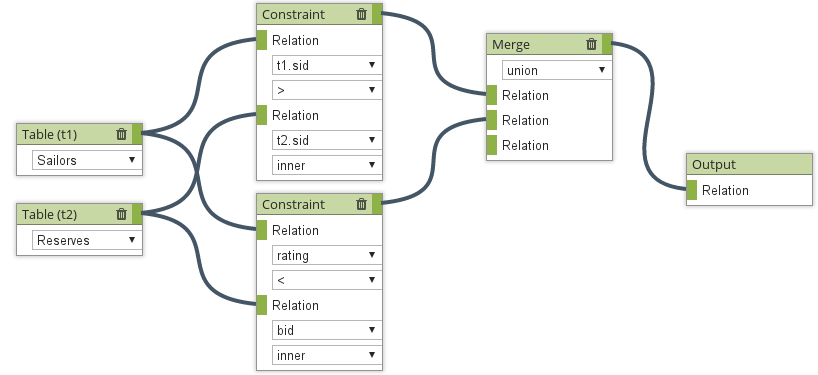
\includegraphics[width=\textwidth]{resources/JoinOR.png}
  \caption{Query featuring a set operator implemented in QENoBI}
  \label{fig:eval_join_or}
\end{figure}

Similarly, some of the queries in the evaluation set require the projection of a large number of columns. While the Select node can handle an infinite number of projections, the node's size increases by a fixed amount with every additional column, eventually becoming unwieldy.

However, the most significant weaknesses revealed by the evaluation are concerned with expressions. Therefore, it appears that the Expression node as specified has a number of shortcomings. First off, as shown before in Listing~\ref{lst:project_constant}, neither the Expression nor the Select node are capable of ``producing columns'', i.e. add new columns that are not based on columns. Interestingly, this issue is closely related to the problem discussed in Section~\ref{sec:issues} that addresses why the projection and aggregation nodes need to be combined. The problem arises due to the fact, that the Select node finalizes a query, making it impossible for the Expression node to modify the columns any further. Unfortunately, the solution applied to the previous issue cannot be used in this case, as combining the interfaces of the nodes into one is infeasible. Additionally, the Expression node cannot handle a variable number of parameters as required by \texttt{CASE} or \texttt{DECODE} expressions. This issue can be easily resolved, but requires a more flexible node architecture than the one used in the current implementation. The reason that these features are missing from the specification is that the original test set failed to cover those cases. This is an obvious limitation of the test set approach. Then again, one reason we used a test set in the first place is that it allows us to focus on the commonly used and therefore most crucial features. As such, considering the limited size of the test set, it is not surprising at all that a number features from the evaluation set are not present in the test set.

%---------------
%Conclusion
%---------------

\chapter{Conclusion}
\label{ch:conclusion}

\section{Conclusion}
\label{sec:conclusion}
The motivation for this thesis was the discontent with existing query builders and the hunch, that by using the concept of dataflow programming, we might be able to conceive a query builder that is not only more powerful but also easier to use. We verbalized this assumption in the research question presented in Section~\ref{sec:res_question}. This thesis provides an answer to this question in the form of the specification of QENoBI, a visual SQL query builder that strives to be as powerful as possible while still being easy to use. To understand the requirements on a powerful query builder, we analyzed a number of existing query builders in Section~\ref{sec:feature_set} and took note of their strengths and weaknesses. The results clearly showed that DFQL, which is based on dataflow programming, is more powerful than the other tools. With the confidence that our motivating hunch was indeed correct, we then started the specification of our query builder by examining different architectures, eventually settling on an approach based on the metaphor of an assembly line. Based on this approach and the requirements found earlier, we then continued to work on the specification by compiling a list of nodes. We then discussed the workings of each individual node, providing us with a first draft version of the specification. At this point, QENoBI is a powerful query builder but we haven't put any thought into usability yet. One of the key aims of QENoBI was to be easy to use for experienced and novice users alike. As such, we needed to abstract enough from SQL to where novice users can construct queries without profound knowledge. At the same time, we also needed to make sure that experienced users are not alienated by the abstraction. Furthermore, to increase the usability for all possible user, the abstraction should simplify query generation both from an understanding \emph{and} efficiency point of view. To address these concerns, we expanded QENoBI by adding subnodes, which can be used to combine the functionality of multiple nodes into one. To verify the concepts, we then implemented a proof-of-concept implementation and evaluated both the implementation and specification on an extended set of test queries. The evaluation showed, the QENoBI is indeed more powerful than any of the other tools. The evaluation also revealed a number of limitations that would have to be addressed in future work. Due to time concerns and the limitations of the implementation of QENoBI, the usability was not evaluated by means of a user study. Overall, QENoBI improves on the current state of the art by supporting more features than any of other query builder tested. Furthermore, it employes a number of techniques targeted at improved usability. Therefore, QENoBI demonstrated that the idea proposed in the itroduction is indeed viable.

\section{Future Work}
\subsection{User Evaluation}
\label{sec:user_eval}
As mentioned in Section~\ref{sec:weaknesses}, usability, one of the main focuses of QENoBI, wasn't properly evaluated in this thesis. The reason for this is that the only way to reliably test the usability of a tool is by conducting a user study, which, due to time constraints, is not a part of this thesis. Nevertheless, this section discusses some possible setups for user studies.

As discussed in Section~\ref{sec:conclusion}, QENoBI is meant to improve usability for all users. Therefore, a user study would have to cover as many users as possible ranging from absolute beginners to expert users. Finding such a group of people can be challenging, as people without knowledge of SQL are likely not particularly interested in the topic either. One great advantage of the current implementation of QENoBI is that it is web-based because it allows for very fast and simple distribution. For instance, to get quick feedback, we could simply post the link online, reaching thousands of people around the globe within minutes therefore greatly increasing the significance of the feedback. To properly assess the usability however, more accurate data is required. For instance, to collect meaningful data on how many queries the average user can implement and how long it takes them, we need to provide a list of assignments to be solved by the users. These assignments should include SQL as well as natural language queries in order to assess the difficulty of translation. Further, we need to be able to establish whether a query was implemented correctly and how long it took a user to do so. In addition, there should also be a questionnaire to address issues that are not expressed in the numbers. To make this less of a hassle, single multiple choice questions could be shown in between assignments with the added possibility to give more detailed feedback on the subject of the question. One way to motivate more users to participate in the assignments is to provide up-to-date statistics. Users could then compare how well they perform against their colleagues, appealing to the natural sense of competitiveness.

The main issue of the approach discussed so far is that it could only show differences between different types of users but not query builders, as QENoBI is the only tool tested. Therefore, to assert the claims made in the research questions, we would have to directly compare how well users perform on the same assignments on different tools. This is tough, as direct comparisons are difficult to implement, especially in the web-based setting described above. The only way to address this issue is to revert to more conventional user study approaches, such as supervised sessions. From a content point of view however, the assignments and questionnaires could be essentially identical.

\subsection{Complete Implementation}
While the implementation discussed in this thesis works well to demonstrate the viability of the concept, it lacks a number of the features described in the specification. Therefore, the logical next step is an implementation that covers the entire specification. This could not be done on the architecture of the proof-of-concept implementation as it is neither powerful nor flexible enough to support subnodes and specifically deferred typing. While an architecture based on the current one could be used, other concepts could be examined as well. For instance, while the proof-of-concept implementation passes information bottom-up, one could imagine an approach that works top-down, i.e. starts at the root. A purely functional implementation would also be highly interesting, due to the close relation of functional programming languages and the dataflow programming paradigm.

\subsection{Extensions}
Currently, QENoBI is limited to generating queries from a single, pre-defined schema and therefore not very practical at all. In order to be of practical use, it would have to be able to handle arbitrary, user-defined schemas or, if possible, even be connected to the database directly.

One of the major advantages of subnodes is that they can be used to abstract on the primitive operators of the relational algebra and SQL. However, in order to be able to create a subnode, the user still needs to understand them. Since QENoBI is a web-application, it would therefore be interesting to implement a feature to share subnodes among users. Using this feature, experienced users could create subnodes such as the Maximize subnode discussed in Section~\ref{sec:subnodes} and provide them to users who are unfamiliar with SQL. This could eventually result in a completely redesigned visual query language that doesn't use any of the primitives nodes but still translates directly into SQL.

\section{Final Words}
In many ways, the process of developing QENoBI turned out to be harder than I expected it to be. Within days of starting the project, I realized that the approach I had in mind wasn't going to work. Upon settling on a new, more powerful approach, I discovered a paper about a dataflow query language, DFQL, which was based on that exact concept. As a result, the focus changed from raw power to a combination of power and usability. Ultimately, I am very happy with the results. The concept of subnodes is very promising and the implementation of this concept in QENoBI is elegant and lightweight but maintains the entire expressiveness of the idea.

\lipsum[1]
\appendix
\chapter{Query Set}
\label{app:test_set}

\section*{Test Set}

\subsection*{Database Management Systems}
\begin{setq}
SELECT *
FROM Sailors
\end{setq}
\begin{setq}
SELECT sname, age
FROM Sailors
\end{setq}
\begin{setq}
SELECT s.sname AS name, s.age
FROM Sailors s
\end{setq}
\begin{setq}
SELECT DISTINCT sname
FROM Sailors
\end{setq}
\begin{setq}
SELECT COUNT(*) AS count
FROM Sailors
\end{setq}
\begin{setq}
SELECT sname, rating+1 AS score
FROM Sailors
\end{setq}
\begin{setq}
SELECT *
FROM Sailors
WHERE rating > 7
\end{setq}
\begin{setq}
SELECT *
FROM Sailors
WHERE rating > 7 AND age < 30
\end{setq}
\begin{setq}
SELECT s.sname
FROM Sailors s JOIN Reserves r ON s.sid = r.sid
\end{setq}

\subsection*{Wikipedia}
\begin{setq}
SELECT
  '&mw_prefix.' || t.table_name table_name,
  t.column_name,
  t.data_default,
  t.data_length,
  t.data_type,
  DECODE (t.nullable, 'Y', '1', 'N', '0') not_null,
  (
    SELECT 1
    FROM
      user_cons_columns ucc,
      user_constraints uc
    WHERE ucc.table_name = t.table_name
      AND ucc.column_name = t.column_name
      AND uc.constraint_name = ucc.constraint_name
      AND uc.constraint_type = 'P'
      AND ROWNUM < 2
  ) prim,
  (
    SELECT 1
    FROM
      user_ind_columns uic,
      user_indexes ui
    WHERE uic.table_name = t.table_name
      AND uic.column_name = t.column_name
      AND ui.index_name = uic.index_name
      AND ui.uniqueness = 'UNIQUE'
      AND ROWNUM < 2
  ) uniq,
  (
    SELECT 1
    FROM
      user_ind_columns uic,
      user_indexes ui
    WHERE uic.table_name = t.table_name
      AND uic.column_name = t.column_name
      AND ui.index_name = uic.index_name
      AND ui.uniqueness = 'NONUNIQUE'
      AND ROWNUM < 2
  ) nonuniq
FROM
  user_tab_columns t,
  user_tables ut
WHERE ut.table_name = t.table_name
\end{setq}
\begin{setq}
SELECT
  fa_id,
  fa_name,
  fa_archive_name,
  fa_storage_group,
  fa_storage_key,
  fa_deleted_user,
  fa_deleted_timestamp,
  fa_deleted_reason,
  fa_size,
  fa_width,
  fa_height,
  fa_metadata,
  fa_bits,
  fa_media_type,
  fa_major_mime,
  fa_minor_mime,
  fa_description,
  fa_user,
  fa_user_text,
  fa_timestamp,
  fa_deleted,
  fa_sha1
FROM
  filearchive;
\end{setq}

\subsection*{Typo3}
\begin{setq}
SELECT *
FROM pages
WHERE pid = 0 
  AND pages.deleted = 0 
  AND pages.hidden = 0 
  AND pages.starttime <= 1281620460 
  AND (pages.endtime = 0 
  OR pages.endtime > 1281620460) 
  AND NOT pages.t3ver_state > 0 
  AND pages.doktype < 200 
  AND (pages.fe_group = ''
  OR pages.fe_group IS NULL 
  OR pages.fe_group = '0' 
  OR ',' || pages.fe_group || ',' LIKE '%,0,%' 
  OR ',' || pages.fe_group || ',' LIKE '%,-1,%')
\end{setq}
\begin{setq}
SELECT
  indexname,
  type,
  columnname
FROM indexcolumns
WHERE tablename = table
ORDER BY indexname, columnno;
\end{setq}

\subsection*{Joomla}
\begin{setq}
SELECT
  CONCAT(
    SUBSTRING_INDEX(
      SUBSTRING(params, LOCATE('filters:', params)),
      '}}', 1
    ),
    '}}'
  ) as filters
FROM '#__extensions' 
WHERE name = 'com_content';
\end{setq}

\subsection*{LedgerSMB}
\begin{setq}
SELECT
  lc.id,
  ec.id
FROM
  entity_class ec CROSS JOIN
  location_class lc
WHERE
  ec.id <> 3 AND
  lc.id < 4;
\end{setq}
\begin{setq}
SELECT
  v_cost,
  v_qty,
  SUM(i.sellprice * i.qty),
  SUM(i.qty)
FROM invoice i
JOIN ap a ON (a.id = i.trans_id)
WHERE i.parts_id = v_parts_id;
\end{setq}
\begin{setq}
SELECT
  v_cost sellprice
FROM
  invoice i JOIN ap a ON (a.id = i.trans_id)
WHERE i.parts_id = v_parts_id
ORDER BY
  a.transdate desc,
  a.id desc
LIMIT 1;
\end{setq}
\begin{setq}
SELECT
  *
FROM
  lsmb13.account_link_description
WHERE
  lsmb13.account_link_description.description NOT IN (
    SELECT
      description
    FROM
      account_link_description
  );
\end{setq}

\subsection*{Microsoft Benchmark}
\begin{setq}
SELECT COUNT(*)
FROM bench B1, bench B2
WHERE B1.KN = 49 AND B1.K250K = B2.K500K
\end{setq}
\begin{setq}
SELECT
  name,
  addr
FROM
  prospects
WHERE
  sex = 'F' AND
  familiy_earn > 40000 AND
  zipcode BETWEEN 02100 AND 12200 AND
  educ = "COLLEGE" AND
  hobby IN ('tennis', 'racquetball');
\end{setq}

\section*{Evaluation Set}

\subsection*{Drupal}
\begin{setq}
SELECT DISTINCT
  fid,
  type,
  title,
  page,
  visibility
FROM profile_field
WHERE name = :name
\end{setq}

\subsection*{WordPress}
\begin{setq}
SELECT COUNT(*)
FROM table
WHERE meta_key = %s
  AND column = %d
\end{setq}
\begin{setq}
SELECT tr.object_id
FROM
  term_relationships AS tr INNER JOIN term_taxonomy AS tt
  ON tr.term_taxonomy_id = tt.term_taxonomy_id
WHERE tt.taxonomy IN (taxonomies)
  AND tt.term_id IN (term_ids)
ORDER BY tr.object_id order
\end{setq}
\begin{setq}
SELECT *
FROM links
WHERE link_id = %d
LIMIT 1
\end{setq}

\subsection*{MusicBrainz}
\begin{setq}
SELECT
  COUNT(id),
  medium
FROM track
GROUP BY medium
\end{setq}
\begin{setq}
SELECT
  entity0 AS event,
  entity1 AS series,
  lrs.id AS relationship,
  link_order,
  lrs.link,
  COALESCE(text_value, '') AS text_value
FROM l_event_series lrs
  JOIN series s ON s.id = lrs.entity1
  JOIN link l ON l.id = lrs.link
  JOIN link_type lt ON (lt.id = l.link_type AND lt.gid = '[...]')
  LEFT OUTER JOIN link_attr_text_value latv
    ON (latv.attr_type = s.ord_attribute AND latv.link = l.id)
ORDER BY
  series,
  link_order;
\end{setq}
\begin{setq}
SELECT
  release,
  date_year,
  date_month,
  date_day,
  country
FROM
  (
    SELECT
      release,
      date_year,
      date_month,
      date_day,
      country
    FROM release_country
    UNION ALL
    SELECT
      release,
      date_year,
      date_month,
      date_day,
      NULL
    FROM release_unknown_country
  ) as q;
\end{setq}

\subsection*{LedgerSMB}
\begin{setq}
SELECT
  id,
  CASE
    WHEN gl.amount = 0
      THEN 0 -- avoid div by 0
    WHEN gl.transdate = ac.transdate
      THEN 1 + sum(ac.amount) / gl.amount
    ELSE 
      1 - (gl.amount - sum(ac.amount)) / gl.amount
  END,
  'ar' as rel,
  ac.transdate
FROM ar gl
JOIN acc_trans ac ON ac.trans_id = gl.id
JOIN account_link al
  ON ac.chart_id = al.account_id
    AND al.description = 'AR'
GROUP BY
  gl.id,
  gl.amount,
  ac.transdate,
  gl.transdate
\end{setq}
\begin{setq}
SELECT
  sum(ac.amount) AS balance,
  e.name, ap.id,
  ap.invnumber,
  ap.transdate,
  ap.taxincluded,
  ap.amount,
  ap.netamount,
  ap.duedate,
  ap.invoice,
  ap.ordnumber,
  ap.curr,
  ap.notes,
  ap.person_id,
  ap.till
FROM ap
 JOIN entity_credit_acc eca ON ap.entity_credit_acc = eca.id
 JOIN entity e ON eca.entity_id = e.id
 JOIN acc_trans ac ON ac.trans_id = ap.id
 JOIN account_link al
   ON al.description = 'AP'
     AND al.account_id = ac.chart_id
GROUP BY
  e.name,
  ap.id,
  ap.invnumber,
  ap.transdate,
  ap.taxincluded,
  ap.amount,
  ap.netamount,
  ap.duedate,
  ap.invoice,
  ap.ordnumber,
  ap.curr,
  ap.notes,
  ap.person_id,
  ap.till
HAVING sum(ac.amount) <> 0;
\end{setq}
\begin{setq}
SELECT
  name,
  'V-' || vendornumber,
  1,
  (
    SELECT
      id
    FROM
      country 
    WHERE
     LOWER(short_name)  = :default_country
  )
FROM
  lsmb12.vendor
GROUP BY
  name,
  vendornumber;
\end{setq}

\subsection*{TPC Benchmark}
\begin{setq}
SELECT
  l_returnflag,
  l_linestatus,
  SUM(l_quantity) AS sum_qty,
  SUM(l_extendedprice) AS sum_base_price,
  SUM(l_extendedprice*(1-l_discount)) AS sum_disc_price,
  SUM(l_extendedprice*(1-l_discount)*(1+l_tax)) AS sum_charge,
  AVG(l_quantity) AS avg_qty, 
  AVG(l_extendedprice) AS avg_price,
  AVG(l_discount) AS avg_disc, 
  COUNT(*) AS count_order
FROM 
  lineitem
WHERE 
  l_shipdate <= date '1998-12-01' - interval '[DELTA]' day (3)
GROUP BY
  l_returnflag, 
  l_linestatus
ORDER BY
  l_returnflag, 
  l_linestatus;
\end{setq}
\begin{setq}
SELECT
  s_acctbal,
  s_name,
  n_name,
  p_partkey,
  p_mfgr,
  s_address,
  s_phone,
  s_comment
FROM
  part, supplier, partsupp, nation, region
WHERE
  p_partkey = ps_partkey
  AND s_suppkey = ps_suppkey
  AND p_size = [SIZE]
  AND p_type LIKE '%[TYPE]'
  AND s_nationkey = n_nationkey
  AND n_regionkey = r_regionkey
  AND r_name = '[REGION]'
  AND ps_supplycost = (
    SELECT
      MIN(ps_supplycost)
    FROM 
      partsupp,supplier, nation, region
    WHERE 
      p_partkey = ps_partkey
      AND s_suppkey = ps_suppkey
      AND s_nationkey = n_nationkey
      AND n_regionkey = r_regionkey
      AND r_name = '[REGION]'
  )
ORDER BY
  s_acctbal desc,
  n_name,
  s_name,
  p_partkey;
\end{setq}
\begin{setq}
SELECT
  o_orderpriority, 
  count(*) as order_count
FROM
  orders
WHERE
  o_orderdate >= date '[DATE]' AND
  o_orderdate < date '[DATE]' + interval '3' month AND
  EXISTS (
    SELECT
      *
    FROM
      lineitem
    WHERE
      l_orderkey = o_orderkey AND
      l_commitdate < l_receiptdate
    )
GROUP BY
  o_orderpriority
ORDER BY
  o_orderpriority;
\end{setq}



\listoffigures
\listoftables
\lstlistoflistings

\chapter*{Acknowledgements}
Foremost, I would like to express my gratitude to my advisor, Christoph Zimmerli, for his support, patience and guidance. I started out with nothing but a rough idea of a tool and through his invaluable input, I was able to transform my idea into this thesis. He found the time to listen to the little problems that cropped up during this process and provided helpful insight in many occasions. I also deeply appreciated his critical feedback and constant motivation.

I would also like to thank Professor Moira Norrie and the entire Information Systems Group at ETH Zurich for all the direct and indirect support and for allowing me to pursue one of my own ideas.

Finally, many thanks go to my fellow computer science students for the inspiring discussions and advice on various problems.

\newpage
\thispagestyle{empty}

\bibliographystyle{plain}
\bibliography{bibliography}

\end{document} 
